\chapter{Group Theory and Special Relativity}
\label{chp:group theory}
Group theory concerns the classification of mathematical similarities between sets of elements and connects these to physical symmetries. 
\paragraph{Definition of a group: }
A set of elements, $a,b,c,...\in G$, is said to form a group if there, between two arbitrary elements of the group, exists a well defined product that satisfies:
\begin{enumerate}
	\item The product of two elements of the group is another element the group $a\cdot b=c$, $\forall a,b:\ni c:a,b,c\in G$.
	\item The group product between several elements is associative, i.e. $a\cdot(b\cdot c)=(a\cdot b)\cdot c$, $\forall a,b,c\in G$.
	\item The identity element exists within the group, i.e. $e\in G$. The identity is defined by the operation on other, generic elements via $a\cdot e=e\cdot a=a$, $\forall a\in G, e\in G$.
	\item There is an inverse to each group element, such that $a^{-1}\cdot a=a\cdot a^{-1}=e$, $\forall a\in G, e\in G$.
\end{enumerate}
\paragraph{An abelian group: }
A group is said to be abelian if the product of group elements is commutative, i.e. $a\cdot b=b\cdot a$, $\forall a,b\in G$.
\paragraph{Order of a group: }
The order of a group is the number of elements in the group.
\paragraph{Subgroup: }
If a subset, $H$, of a group, $G$, fulfill the requirements for a group, then the subset forms a subgroup.
\paragraph{Continuous group: }
If the group elements carry a label, which is a continuous parameter, the group is said to be continuous. A continuous group of special interest to physics is the Lie group\index{Lie group}. A Lie group is a group which is also a differentiable manifold\index{Manifold}. In mathematics, a manifold is a topological space that locally resembles Euclidean space near each point. This means that a geometrical structure can be associated with Lie groups and the group can be associated with such a structure in some abstract space. Further more, the elements of a Lie group must be parameterized smoothly and continuously.
\begin{example}
	\begin{enumerate}
		\item The general linear group, of dimension $n$, $GL(n)$, can be represented as the set of all invertible $n\times n$ matrices.
		\item The unitary group, of dimension $n$, $U(n)$, can be represented as the set of $n\times n$ unitary matrices. Ie. matrices satisfying $UU^\dagger=U^\dagger U=I$.
		\item The special unitary group, of dimension $n$, $SU(n)$, can be represented as the set of unitary matrices with unit determinant.
		\item The orthogonal group, of dimension $n$, $O(n)$, can be represented as the set of real, orthogonal matrices. Ie. matrices satisfying $M^T=M^{-1}$. The different groups are connected via the relation
		\begin{equation}
			SU(n)\wedge O(n)\in U(n)\in GL(n).
		\end{equation} 
		The relationship is also seen illustrated in figure \ref{fig:2}.
		\begin{figure}[h]
			\captionsetup{width=1\textwidth}
			\centering
			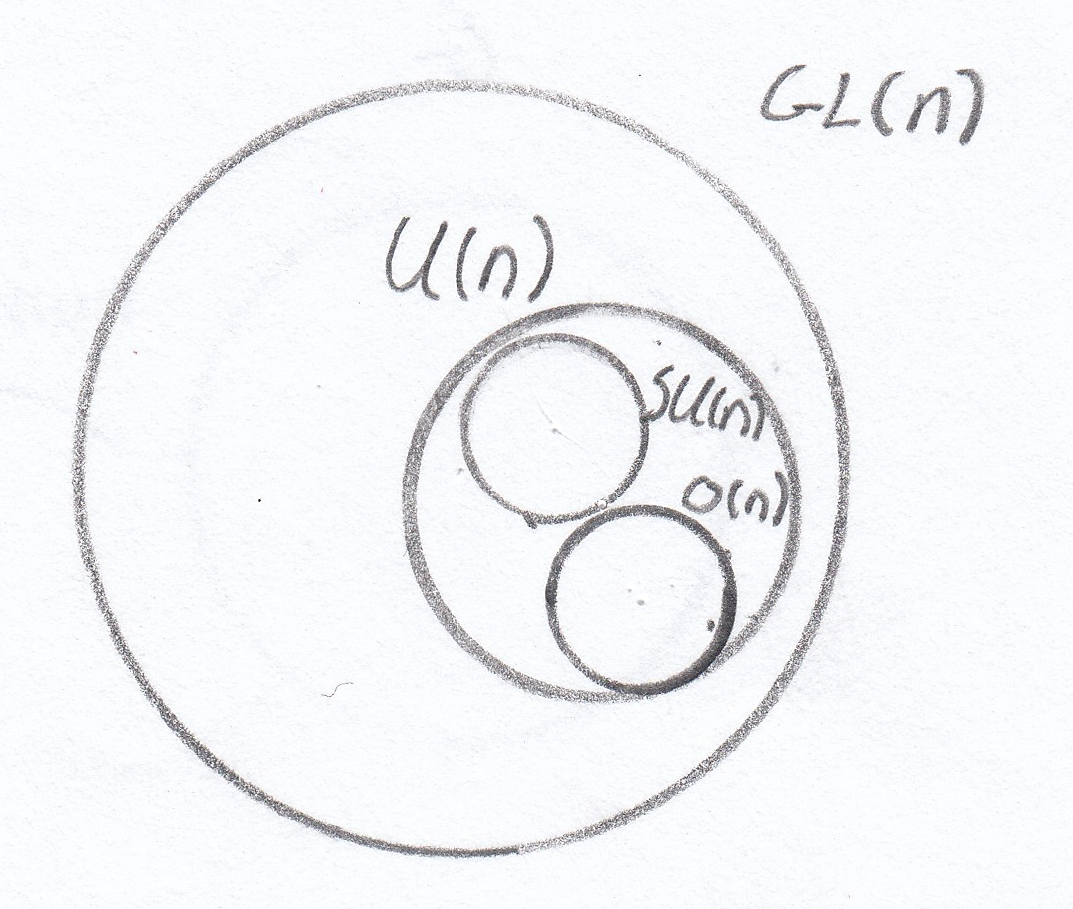
\includegraphics[width=0.4\textwidth]{figures//2}
			\caption{The relationship between the different groups mentioned above.}
			\label{fig:2}
		\end{figure}
	\end{enumerate}
\end{example}

\paragraph{Homomorphism: }
A homomorphism is a mapping between two groups, $G$ and $G'$, that conserve group multiplication. The map does not have to be one-to-one. An illustration of the mapping is seen in figure \ref{fig:3}.
\begin{figure}[h]
	\captionsetup{width=1\textwidth}
	\centering
	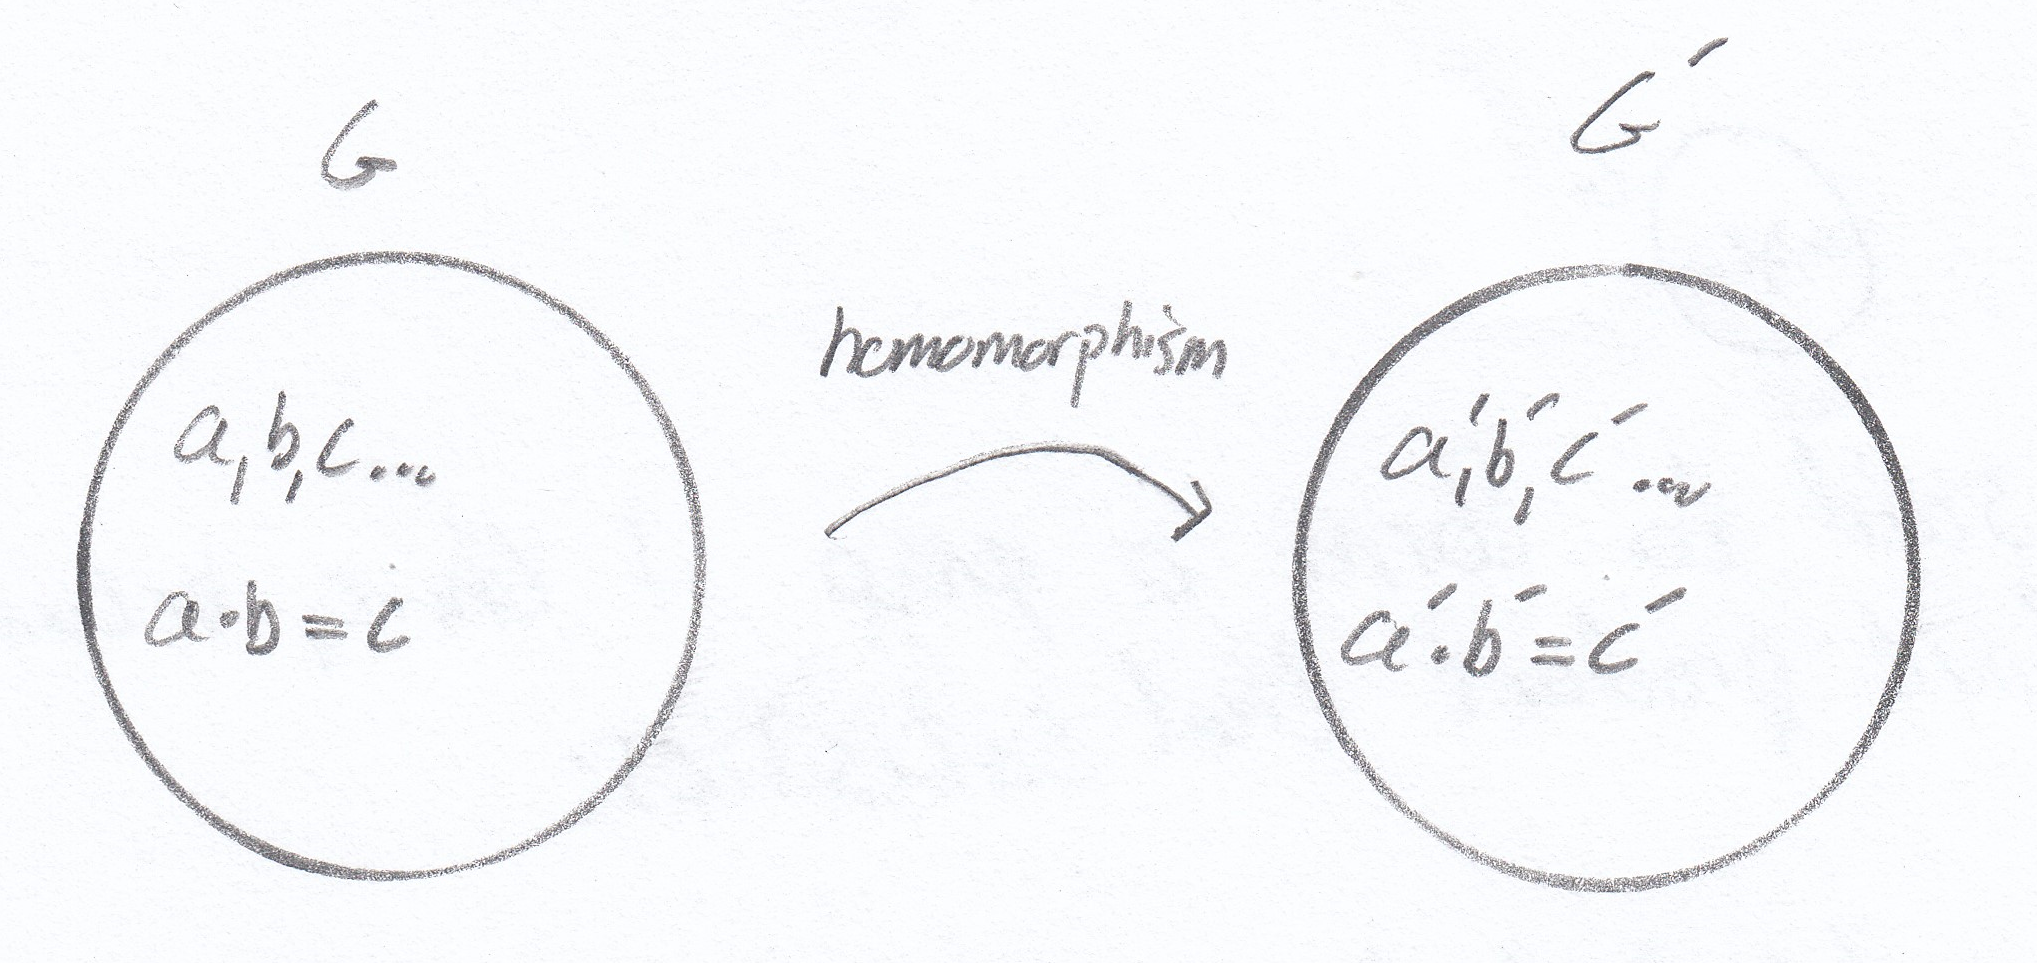
\includegraphics[width=0.5\textwidth]{figures//3}
	\caption{An illustration of a homomorphism between two groups.}
	\label{fig:3}
\end{figure}

\paragraph{Isomorphism: }
An isomorphism is a homomorphism between two groups, $G$ and $G'$, with a one-to-one correspondence. Hence, not only group multiplication is preserved, but also
\begin{equation}
	a \rightleftarrows a', \quad b \rightleftarrows b', \quad  c \rightleftarrows c',...
\end{equation}  
\paragraph{Conjugate elements of a group: }
Elements of a group, $G$, $a,b\in G$, is said to be conjugate to each other if there exist another element, $p\in G$, such that $b=pap^{-1}$.
\paragraph{Direct product group: }
Let $H_1$ and $H_2$ be subgroups of $G$ which satisfies:
\begin{enumerate}
	\item All elements of $H_1$ and $H_2$ commute, i.e. $h_1h_2=h_2h_1$, $\forall h\in H_1 \wedge h_2\in H_2$.
	\item All elements of $G$ can be described as the product of an element from $H_1$ and an element from $H_2$. Ie. $h_1h_2=g\in G, \forall g$. 
\end{enumerate}
In this case $G$ is said to be the direct product of $H_1$ and $H_2$. This is denoted by $G=H_1\otimes H_2$.
\paragraph{Group representation: }
If there is a homomorphism\footnote{A homomorphic representation is called unfaithful whereas an isomorphic representation is called faithful.} from a group, $G$, to a set of operators, $U(g)$ (where $g$ are the group elements of $G$), defined on a linear vector space, $V$, then $U(g)$ is a representation\footnote{Informally the representation of a group is a way of writing the group as matrices.} of $G$. The concept of a representation is shown in figure \ref{fig:4}.
\begin{figure}[h]
	\captionsetup{width=1\textwidth}
	\centering
	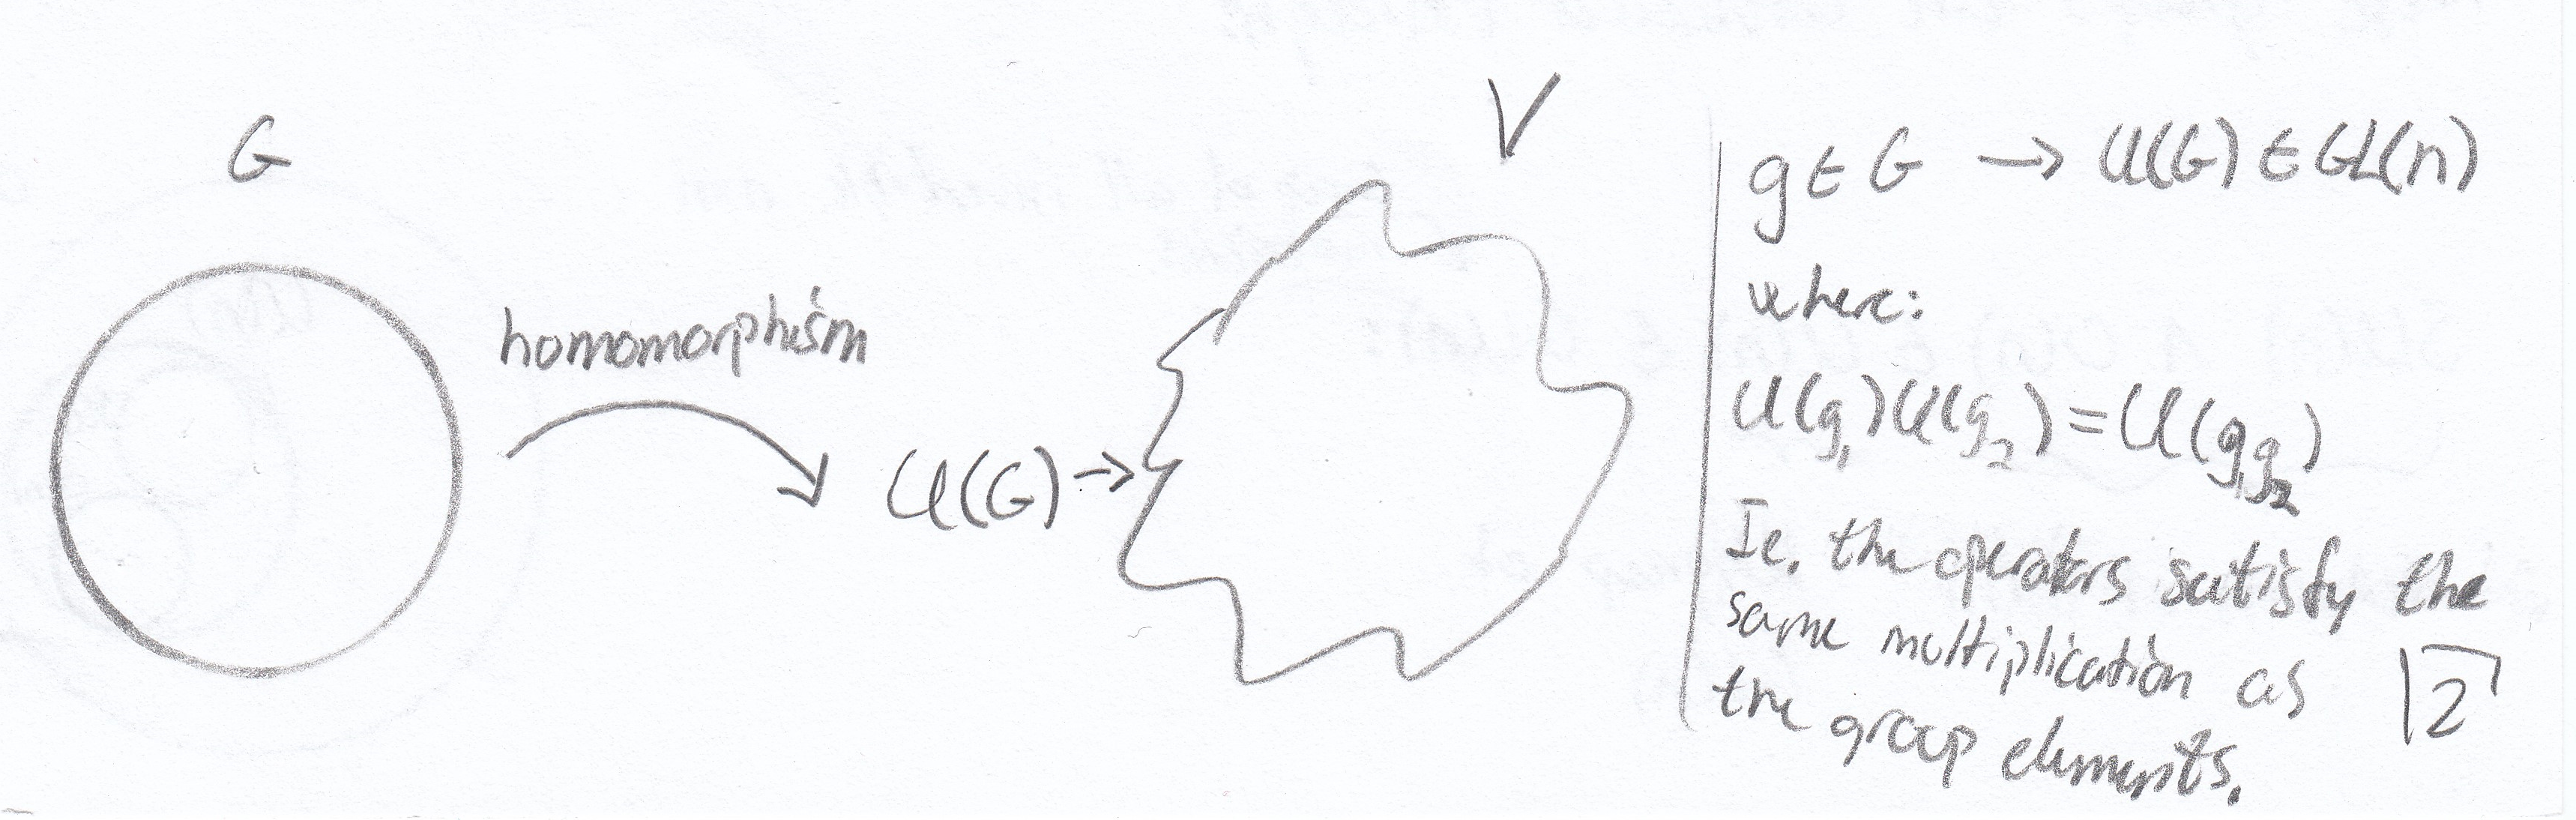
\includegraphics[width=0.6\textwidth]{figures//4}
	\caption{An illustration of a representation of a group.}
	\label{fig:4}
\end{figure} 
In terms of representations of Lie groups it is important to remember that a Lie group is defined in terms of the associated manifold. For this reason one can talk about different representations of groups made up by matrices\footnote{It is a confusing thought to think of representing matrices of a given dimension by other matrices with different dimensions. However, one should think of it like this; a given Lie group has an associated manifold. This manifold can have several representations. For example; $SU(2)$ is the group of $2\times 2$ unitary matrices with unit determinant. The manifold of this group is a circle. The manifold can be represented by either $2\times 2$ matrices or complex number (as is commonly done with the unit circle in complex space).} (eg. $SU(2)$). The representation of a Lie group is a representation of the associated manifold.

\paragraph{Invariant subspace:}\index{invariant subspace} Consider a representation, $U(g)$, of a group, $G$, defined on a linear vector space $V$. $V'\subseteq V$ is called an invariant subspace if for $v\in V'$; $U(g)v\in V'$, $\forall g\in G$. This means that if a vector in the invariant subspace $V'$ act on an arbitrary group element the transformed vector will always be again a part of the invariant subspace, $V'$. For an invariant subspace a representation $U'(g)$ of $G$ on $V'$, called a sub-representation of $U(g)$, can be defined viz
\begin{equation}
	U'(g)v=U(g)v,\quad \forall v\in V'.
\end{equation} 
This leads to the notion that the representation $U(g)$ is not a fundamental but instead composed of smaller building blocks. 

\paragraph{Irreducible representations:} An irreducible representation\index{Irreducible representation} is a representation of a group $G$ on a vector space $V$ that has no invariant subspaces besides $0$ and $V$ itself. Such representations can be thought of as truly fundamental since they are not made up of smaller representations. The irreducible representations of a group are the building blocks from which any other representation of the group can be built. A different approach to irreducible representations can be found by considering similarity transformations\index{Similarity transformation}. Given a matrix, $R$, and an invertible matrix, $S$, the similarity transformation is defined viz
\begin{equation}
	R\Rightarrow R'=S^{-1}RS.
\end{equation} 
If $R$ is a representation of the group $G$, then so is $R'$. An irreducible representation can be defined as a representation that cannot be transformed into block diagonal form via a similarity transformation.  

\paragraph{Generators of a discrete group: }
\index{Generators of a discrete group}
A collection, $c$, of elements of a discrete group, $G$, is said to be generators of the group if multiplication among the generators yield all elements of the group. 
\paragraph{Generators of a continuous group: }
\index{Generators of a continuous group}
In the case of a continuous group the generators are defined different, compared to the discrete group, since there are no single elements in a continuous group, but a continuum of elements. Consider a set of elements, $R$, that depends on some real, continuous parameters
\begin{equation}
	R=R(x,y,z,...).
\end{equation} 
These elements form a continuous group if $R$ fulfil the requirements for a group. If $R$ is differentiable, the group is a Lie group. Differentiability means that $R(dx)$ only differs infinitesimally from $R(0)=e$ by a term od order $dx$. Therefore $R(dx)$ can be parametrized as
\begin{equation}
	R(dx)=e-idxJ,
	\label{dj}
\end{equation} 
where $e$ is the identity element, the "$-i$" is included by convention (to make $J$ Hermitian) and $J$ is \emph{defined} as the generator of the group. By going from $dx\Rightarrow x$
\begin{equation}
	R(x)=\lim\limits_{N\Rightarrow \infty}\bigg(e-i\frac{dxJ}{N}\bigg)^N=e^{-ixJ}.
	\label{eq8}
\end{equation} 
In the considered case, used for illustrative purposes, there is only one parameter ($x$) and one corresponding generator ($J$). In general, a group can have several parameters ($\alpha_i$) and corresponding generators ($t_i$). The different generators make up a vector space. This vectors space is called a Lie algebra. 
\paragraph{Lie algebra:} A Lie algebra is a vector space, $\texttt{g}$, equipped with a binary operation (called the Lie bracket\footnote{The Lie bracket is often called the Lie algebra.}), $[,]: \texttt{g}\times \texttt{g}\Rightarrow \texttt{g}$. The binary operation satisfies the following axioms:
\begin{enumerate}
	\item Bilinearity:$[aX+bY,Z]=a[X,Z]+b[Y,Z]$ and $[Z,aX+bY]=a[Z,X]+b[Z,Y]$, for arbitrary numbers $a,b$ and $\forall X,Y,Z\in \texttt{g}$.
	
	\item Anticommutativity: $[X,Y]=-[Y,X]$ $\forall X,Y\in \texttt{g}$.
	
	\item The Jacobi identity: $[X,[Y,Z]]+[Z,[X,Y]]+[Y,[Z,X]]=0$ $\forall X,Y,Z \in \texttt{g}$. 
\end{enumerate}
The Lie algebra is therefore a vector space consisting of the generators of a Lie group. However, it is important to note that the definition of the Lie algebra makes no reference to any Lie group. Therefore the definition stands on its own and therefore one can talk about different Lie groups having the same Lie algebra. This leads to the definition of a distinguished Lie group.
\paragraph{Distinguished Lie group:} There is precisely one distinguished Lie group for each Lie algebra. The distinguished group has the property of being simply connected. This means that any closed curve on the manifold, corresponding to the Lie group, can be shrunk smoothly to a point. The simply connected group can be thought of as the "mother" of all those groups having the same Lie algebra, because there are maps to all other groups with the same Lie algebra from the simply connected group, but not vice versa. An intuitive name could be the "mother" group of a given Lie algebra. Formally the group is called the \emph{covering group}. All other groups with the same Lie algebra is said to be covered by the simply connected group.

\begin{example}
	Consider the group $SO(2)$. It is a one dimensional group describing rotations in $2$ dimensions. The group is one dimensional since only one continuous parameter, $\theta$, characterizes a rotation. The elements of the group can be represented by $2\times 2$ matrices which commute, and so the group is an abelian group. The group has one generator, $L$, which can be used to generate all elements of the group via
	\begin{equation}
		R(\theta)=e^{-i\theta L}.
	\end{equation} 
	Since the group is designated by $SO(2)$ each matrix is orthogonal an have unit determinant. 
\end{example}
\begin{example}
	This example will consider the isomorphism between $U(1)$ and $SO(2)$. As mentioned in example $4.2$ $SO(2)$ describes rotations in two dimensions and the group elements can be represented, in terms of the generator $L$, as
	\begin{equation}
		R(\theta)=e^{-i\theta L}.
	\end{equation} 
	$U(1)$ is the manifold of unitary $1\times 1$ matrices, i.e. unit complex numbers. The generator of the groups is the identity, $e$, and so the elements can be represented as
	\begin{equation}
		R(x)=e^{-ix}
	\end{equation} 
	There is an isomorphism between the two groups. This can be shown by considering
	\begin{equation}
		R(\theta_1)R(\theta_2)=e^{-i\theta_1 L}e^{-i\theta_2 L}=e^{-i(\theta_1+\theta_2) L}=R(\theta_1+\theta_2),
	\end{equation} 
	\begin{equation}
		f(x_1)f(x_2)=e^{-ix_1}e^{-ix_2}=e^{-i(x_1+x_2)}=f(x_1+x_2).
	\end{equation} 
	It is clear that there is a one-to-one correspondence between $x$ and $\theta$, and so $U(1)$ and $SO(2)$ are isomorphic to each other. The manifold associated with unit complex numbers is the unit circle in the complex plane. Since there is an isomorphism between $U(1)$ and $SO(2)$,the manifold of $SO(2)$ is likewise the unit circle in the complex plane. Hence, one can think of the Lie group as being the unit circle and the manifestation of the elements in complex numbers ($U(1)$) and matrices ($SU(2)$) as representations of the manifold. 
\end{example}


\section{$SO(3)$}
The group $SO(3)$ manifold corresponding to orthogonal $3\times 3$ matrices with unit determinant. The geometric shape of the manifold will be considered in the next section (on $SU(2)$). The reason for this is that $SU(2)$ is the simply connected group of the Lie algebra which it shares with $SO(3)$. Hence, the manifold of $SO(3)$ is a part of the manifold of $SU(2)$.\newline
The matrices describe rotations in $3d$ space. Formally; the $SO(3)$ group consists of all continuous, linear transformations in $3d$ Euclidean space which leave the length of coordinate vectors invariant. The elements of $SO(3)$ does not, in general, commute and so $SO(3)$ is, as opposed to eg. $U(1)$ or $SO(2)$, a non-abelian Lie group.\newline
A generic rotation in $3d$ is parametrized by $3$ rotations, by $3$ continuous angles, around the three coordinate axis. Corresponding to each continuous parameter is a generator, and so $SO(3)$ has $3$ basis generators. The rotations around a given axis form a subgroup of $SO(3)$ that is isomorphic to $SO(2)$. Since there are $3$ coordinate axis' there are $3$ basis generators, denoted by $J_i$. the Lie bracket of the generators is given by
\begin{equation}
	[J^i,J^j]=i\epsilon^{ijk}J^k.
\end{equation} 
From the basis generators a generic element of $SO(3)$ can be described as
\begin{equation}
	R(\alpha,\beta,\gamma)=R_3(\gamma)R_2(\beta)R_1(\alpha)=e^{-iJ_3\gamma}e^{-iJ_2\beta}e^{-iJ_1\alpha},
\end{equation} 
where $\alpha,\beta,\gamma$ are \emph{Euler angles} and the basis matrices $R_i$ are given by
\begin{equation}
	\begin{split}
		&R_1(\alpha)=\begin{bmatrix}
			1 & 0 & 0 \\
			0 & cos(\alpha) & sin(\alpha)\\
			0 & -sin(\alpha) & cos(\alpha)\\
		\end{bmatrix},\\
		& 
		R_2(\beta)=\begin{bmatrix}
			cos(\beta) & 0 & -sin(\beta) \\
			0 & 1 & 0\\
			sin(\beta) & 0 & cos(\beta)\\
		\end{bmatrix},\\
		& 
		R_3(\gamma)=\begin{bmatrix}
			cos(\gamma) & sin(\gamma) & 0 \\
			-sin(\gamma) & cos(\gamma) & 0\\
			0 & 0 & 1\\
		\end{bmatrix},
	\end{split}
	\label{rot}
\end{equation} 
where $R_i$ rotate the coordinate system, not the vector. It is a choice of convention. Rotating the vector is called an active transformation whereas rotating the coordinate system is called a passive transformation. Since the placement of a coordinate system is entirely up to the physicist, i.e. the coordinate system is not a physical thing, it makes more intuitive sense to alternate your definition than actually going in and rotating the physical vector. Hence, here the approach of passive transformations is used.

\section{$SU(2)$}
The group $SU(2)$ is manifold corresponding to unitary $2\times 2$ matrices with unit determinant. The manifold of $SU(2)$ is found by extending the method used to discover the manifold of $SO(2)$. In discovering the manifold of $SO(2)$ it was used that $SO(2)$ is isomorphic to $U(1)$, i.e. sharing manifold, and that $U(1)$ consists of two dimensional complex, unitary numbers which are defined on the unit circle in the complex plane. Extending this analogy the manifold of $SU(2)$ can be found as the manifold of 4 dimensional complex, unitary numbers; quaternions. To describe 4 dimensional complex numbers three imaginary units are needed - As opposed to one imaginary unit for two dimensional complex numbers ($i$). The three imaginary units are defined viz
\begin{equation}
	i^2=j^2=k^2=ijk=-1.
\end{equation} 
Then a 4 dimensional complex number, a quaternion, can be parametrized viz
\begin{equation}
	q=a+bi+cj+dk.
\end{equation} 
The set of unit quaternions are those that satisfy
\begin{equation}
	qq^\dagger=a^2+b^2+c^2+d^2=1.
\end{equation} 
Just as complex numbers can be represented as matrices by mapping the complex unit ($i$) to a matrix, so can quaternions. Specifically~\citep{Schwichtenberg2015}
\begin{equation}
	I=\begin{bmatrix}
		1 & 0\\
		0 & 1\\
	\end{bmatrix}, \quad \hat{i}=\begin{bmatrix}
		i & 0 \\
		0 & -i \\
	\end{bmatrix}, \quad \hat{j}=\begin{bmatrix}
		0 & 1\\
		-1 & 0 \\
	\end{bmatrix}, \quad \hat{k}=\begin{bmatrix}
		0 & i \\
		i & 0 \\
	\end{bmatrix}.
\end{equation} 
This means the generic quaternion can be parametrized viz
\begin{equation}
	q=aI+b\hat{i}+c\hat{j}+d\hat{k}=\begin{bmatrix}
		a+ib & c+id\\
		-c+id & a-ib\\
	\end{bmatrix}\Rightarrow det(q)=a^2+b^2+c^2+d^2.
	\label{as}
\end{equation} 
Comparing equation \eqref{as} to the definition of unit quaternions ($qq^\dagger=1$), it is clear that the matrices must be unitary and have unit determinant. That is the matrices make up the group $SU(2)$. Hence, unit quaternions are isomorphic to $SU(2)$ just like $U(1)$ is isomorphic to $SO(2)$. Hence, the manifold of $SU(2)$ can be described by the unit quaternions. The unit quaternions are characterized by $a^2+b^2+c^2+d^2=1$, analogous to how 2 dimensional unit complex numbers are characterized by $z=a+ib\Rightarrow a^2+b^2=1$. $a^2+b^2=1$ describes the unit circle, $S^1$. Hence, the manifold of two dimensional unit complex numbers is the unit circle in the complex plane. Likewise $a^2+b^2+c^2+d^2=1$ describes the unit three sphere, $S^3$. Hence, the manifold of four dimensional unit complex numbers is the unit three sphere. The unit three sphere is a simply connected manifold. Hence, $SU(2)$ is simply connected.

\subsection{Relationship between $SO(3)$ and $SU(2)$}
To relate the two groups it will be investigated how quaternions can be used to rotate a vector. Parametrizing a vector viz
\begin{equation}
	v=v_x\hat{i}+v_y\hat{j}+v_z\hat{k}=\begin{bmatrix}
		iv_x & v_y+iv_z\\
		-v_y+iv_z & -iv_x\\
	\end{bmatrix}\Rightarrow det(v)=x^2+y^2+z^2.
	\label{as4}
\end{equation} 
The determinant of $v$ is the length of the vector. Since the length of a vector is conserved during a rotation, the transformation must preserve determinants. This means restricting ourselves to unit quaternions as a means to transform the vector
\begin{equation}
	v\Rightarrow v'=q^{-1}vq,
	\label{as1}
\end{equation} 
where once again the approach of passive transformations has been applied. The inverse transformation, $qvq^{-1}$, is the corresponding active rotation\footnote{$qvq^{-1}$ is just a the inverse transformation of $q^{-1}vq$. This makes intuitively sense since rotating a vector in one direction is equivalent to rotating the coordinate system in the opposite direction. Hence, the definition of active and passive rotations is related to the definition of positive and negative angles also.}. In order to relate the transformation of equation \eqref{as1} to rotations the rotation angles must be introduced. In this regard it is convenient to parametrize the unit quaternion viz
\begin{equation}
	q=cos(\theta)+sin(\theta)||\vec{e}||,
\end{equation} 
where $||\vec{e}||$ is the normalized rotation axis. For transparency consider a rotation of $\frac{\vec{x}}{|\vec{x}|}\equiv \hat{x}$ around the $z$-axis. In this case
\begin{equation}
	q=cos(\theta)I+sin(\theta)k=\begin{bmatrix}
		cos(\theta) & isin(\theta)\\
		isin(\theta) & cos(\theta)\\
	\end{bmatrix}.
	\label{as2}
\end{equation} 
Using equation \eqref{as2}
\begin{equation}
	q^{-1}\hat{i}q=\begin{bmatrix}
		cos(\theta) & -isin(\theta)\\
		-isin(\theta) & cos(\theta)\\
	\end{bmatrix}\begin{bmatrix}
		i & 0\\
		0& -i\\
	\end{bmatrix}\begin{bmatrix}
		cos(\theta) & isin(\theta)\\
		isin(\theta) & cos(\theta)\\
	\end{bmatrix}=\begin{bmatrix}
		icos(2\gamma) & -sin(2\theta)\\
		sin(2\theta) & -icos(2\theta)\\
	\end{bmatrix}.
	\label{as3}
\end{equation} 
Comparing equation \eqref{as3} to equation \eqref{as4}
\begin{equation}
	\begin{split}
		&v_x\Rightarrow v'_x=cos(2\theta),\\
		&v_y\Rightarrow v'_y=-sin(2\theta),\\
		&v_z\Rightarrow v'_z=0.\\
	\end{split}
	\label{as5}
\end{equation} 
Rotating a vector in 3-space reveals, cf. equation \eqref{rot}
\begin{equation}
	R_3(\gamma)\hat{x}
	\begin{bmatrix}
		cos(\gamma) & sin(\gamma) & 0 \\
		-sin(\gamma) & cos(\gamma) & 0\\
		0 & 0 & 1\\
	\end{bmatrix}\begin{bmatrix}
		1\\0 \\0\\
	\end{bmatrix}=\begin{bmatrix}
		cos(\gamma)\\
		-sin(\gamma)\\
		0\\
	\end{bmatrix}.
	\label{as6}
\end{equation} 
By comparing equation \eqref{as5} and \eqref{as6} it is clear that $\gamma=2\theta$. That is, in rotating $\hat{x}$ by $\theta$ the vector is rotated by $2\gamma$ in 3-space. This means that there is a two-to-one map from the manifold of $SU(2)$ to the manifold of $SO(3)$, i.e. there are two elements in the manifold of $SU(2)$ that corresponds to the same element in the manifold of $SO(3)$. Hence given one element of the manifold of $SU(2)$ one can find the corresponding element in the manifold of $SO(3)$ but not vice versa. this confirms that the manifold of $SU(2)$ is indeed simply connected. Since there is a two-to-one correspondence between the manifolds of $SU(2)$ and $SO(3)$, and the manifold of $SU(2)$ is the unit three sphere, the manifold of $SO(3)$ must be half a unit three sphere. Since the manifold of $SU(2)$ covers the manifold of $SO(3)$ twice it is called the double cover of the manifold of $SO(3)$.

\section{The Lorentz group}
\label{sec:lor}
The Lorentz group\index{The Lorentz group}, denoted by\footnote{Three space-like dimensions and one time-like dimension.} $O(3,1)$, is the group representing the coordinate transformations of $SR$; boosts and rotations that is. Because the Lorentz group describes the transformations of SR, which are transformations of four vectors, the Lorentz groups is often analysed in a certain representation; the vector representation. In the vector representation an event in SR is described by a four vector on the form
\begin{equation}
	x^\mu\equiv \begin{bmatrix}
		t \\
		\vec{x}\\
	\end{bmatrix}.
\end{equation} 
This vector is called contravariant (index up) and it is defined by its transformation properties
\begin{equation}
	dx^\mu\Rightarrow d{x'}^\mu=\underbrace{\frac{\partial {x'}^\mu}{\partial x^\nu}}_{\Lambda^\mu_{\,\,\,\nu}}dx^\nu.
	\label{contra}
\end{equation} 
Any vector that transforms in this way is called a contravariant vector. Likewise, a covariant vector is defined by
\begin{equation}
	dx_\mu\Rightarrow d{x'}_\mu=\underbrace{\frac{\partial {x'}_\mu}{\partial x_\nu}}_{(\Lambda^{-1})^\nu_{\,\,\,\mu}=\Lambda_\mu^{\,\,\,\nu}}dx_\nu.
\end{equation} 
The contra-variant and covariant vectors are related by the metric via
\begin{equation}
	x^\mu=g^{\mu\nu}x_\nu.
\end{equation} 
During the coordinate transformations, the length of the vectors, $x^\mu x_\mu\equiv x\cdot x=x^2$, is invariant. The length of a vector can be expressed via the metric
\begin{equation}
	x^\mu x_\mu=g_{\mu\nu}x^\mu x^\nu=g_{\mu\nu}x'^\mu x'^\nu=g_{\mu\nu}\Lambda^\nu_{\,\,\,\,\alpha}\Lambda^\mu_{\,\,\,\,\beta}x^\alpha x^\beta.
\end{equation} 
Rearranging the dummy indices
\begin{equation}
	g_{\mu\nu}x^\mu x^\nu=g_{\alpha\beta}\Lambda^\alpha_{\,\,\,\nu}\Lambda^\beta_{\,\,\,\mu}x^\nu x^\mu\Rightarrow g_{\mu\nu}=g_{\alpha\beta}\Lambda^\alpha_{\,\,\,\nu}\Lambda^\beta_{\,\,\,\mu},
\end{equation} 
which can be written $g=\Lambda^Tg\Lambda$ in matrix notation. Taking the determinant, and using that $g_{\mu\nu}=\eta_{\mu\nu}=diag(1,-1,-1,-1)$ for Minkowski space
\begin{equation}
	det(\eta)=det(\Lambda^T)det(\eta)det(\Lambda)\Rightarrow det(\Lambda^T)det(\Lambda)=1.
\end{equation} 
Use now that $det(\Lambda^T)=det(\Lambda)$ to find $det(\Lambda)^2=1\Rightarrow det(\Lambda)=\pm 1$. Transformations for which $det(\Lambda)= 1$ are called proper. Transformations for which $det(\Lambda)= -1$ are called improper. Another classification comes from
\begin{equation}
	g_{00}=1=\Lambda^\alpha_{\,\,\,0}\Lambda^\beta_{\,\,\,0}g_{\alpha\beta}=(\Lambda^0_{\,\,\,0})^2-\sum_{i=1}^{3}(\Lambda^i_{\,\,\,0})^2\Rightarrow |\Lambda^0_{\,\,\,0}|>1.
\end{equation} 
This allows $\Lambda^0_{\,\,\,0}>1$ or $\Lambda^0_{\,\,\,0}<-1$. The transformations characterized by $\Lambda^0_{\,\,\,0}>1$ are called orthochronous whereas transformations characterized by $\Lambda^0_{\,\,\,0}<-1$ are called non-orthochronous. Hence, the Lorentz transformations can be grouped into $4$ categories\footnote{That this is correct can be seen by considering the $TP\Lambda^{po}$-term; the determinant must be positive since it is proper. The determinant of $\Lambda^{po}$ is defined as positive and since the determinant is distributive and negative for both $T,P$, the table must be as shown. The table is confirmed by \citet{Srednicki2027}.} shown in figure \ref{fig:5}.
\begin{figure}[H]
	\captionsetup{width=1\textwidth}
	\centering
	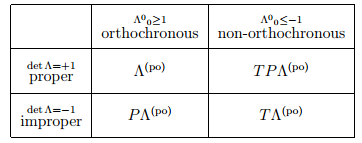
\includegraphics[width=0.4\textwidth]{figures//5}
	\caption{The different categories of Lorentz transformations.}
	\label{fig:5}
\end{figure} 
As shown in figure \ref{fig:5} the different elements of the categories can all be expressed in terms of proper, orthochronous transformations followed by a time-inversion and/or parity operation. Parity is called the "mirror-transformation". Until 1956 physicists believed all physical systems should be invariant under parity. However, in 1956 it was found that the weak interaction violates parity. Mathematically, parity is expressed viz
\begin{equation}
	\Lambda_P x=\begin{bmatrix}
		t\\
		-\vec{x}\\
	\end{bmatrix}, \quad \text{and} \quad  \Lambda_Pp=\begin{bmatrix}
		p^0\\
		-\vec{p}\\
	\end{bmatrix},
\end{equation} 
where $\Lambda_P=diag(1,-1,-1,-1)$ in the vector representation\footnote{Not in general, only in the vector representation.}. Similarly, time-inversion is given by
\begin{equation}
	\Lambda_T x=\begin{bmatrix}
		-t\\
		\vec{x}\\
	\end{bmatrix}, \quad \text{and} \quad  \Lambda_Tp=\begin{bmatrix}
		-p^0\\
		\vec{p}\\
	\end{bmatrix},
\end{equation} 
where $\Lambda_T=diag(-1,1,1,1)$ in the vector representation\footnote{Not in general, only in the vector representation.}. Since the subsets that are not elements of the proper orthochronous subgroup can be determined via applying parity and/or time-inversion, the elements of the proper, orthochronous subgroup is of special interest. Since all elements of the Lorentz group is enclosed in $O(3,1)$, and proper means $det(\Lambda)=1$, the proper, orthochronous transformations (indeed all proper transformations) are members of $SO(3,1)$- in this case a subgroup of $O(3,1)$. $SO(3,1)$ is also called the proper Lorentz group, but most often it is just referred to as the Lorentz group. $SO(3)$ consists of all boost, rotations and combinations of the two. A generic element of the proper, orthochronous subgroup of the Lorentz group can therefore be expressed as
\begin{equation}
	\Lambda^\mu_{\,\,\,\nu}=\Lambda(R')^\mu_{\,\,\,\alpha}\Lambda(\gamma)^\alpha_{\,\,\,\beta}\Lambda(R)^\beta_{\,\,\,\nu}.
\end{equation} 
The $\Lambda$-matrices form a representation of the Lorentz group.

\begin{example}
	\index{4-vector}
	\index{Current density}
	\index{Four current}	
	\emph{Prove that $J^\mu$ is a $4$-vector, where}\newline
	\begin{equation}
		J^\mu=\begin{bmatrix}
			\rho\\
			J_x\\
			J_y\\
			J_z\\
		\end{bmatrix}=\begin{bmatrix}
			\rho\\
			\rho v_x\\
			\rho v_y\\
			\rho v_z\\
		\end{bmatrix}=\begin{bmatrix}
			\rho\\
			\vec{J}\\
		\end{bmatrix}.
	\end{equation} 
	An $n$-dimensional vector is a physical object that can be represented as a $n\times1$ matrix. Because a vector can be represented as a matrix, it must obey the rules of linear algebra, including scalar multiplication, vector addition, dot product, scalar and vector projections. Further more a vector is a rank 1 tensor, which means that it must transform in a well defined way during a coordinate transformation; it must conserve its length during a coordinate transformation. This last definition will be used to verify that $J^\mu$ is in fact a 4-vector. For a $4$-vector the length is called the spacetime interval ($ds^2$). Consider a volume ($V_1$) of charge moving with a uniform velocity ($v_{1x}$) as observed from the reference frame $S_1$\footnote{I only consider movement along the $x$-axis to illustrate the principle. A general treatment is rather cumbersome.}. In this frame the spacetime interval will be given by
	\begin{equation}
		ds_1^2=\rho_1^2(v_{1x}^2-1),
	\end{equation} 
	where the $y$ and $z$ components of the velocity is zero and the subscript on $ds_1$ is introduced because current density has not been proven a $4$-vector yet (and therefore that $ds$ for different reference frames is the same). From $S_1$ the volume containing the charge is contracted via.
	\begin{equation}
		V_1=\gamma^{-1}(v_{1x})V_0,
	\end{equation} 
	where $\gamma=\gamma(v)=(1-v^2)^{-\frac{1}{2}}$. The volume is contracted in the direction parallel to the direction of motion, and hence the volume is diminished as seen from $S_1$. Considering the scenario from the reference frame of $S_2$, which moves with a uniform velocity $v$ with respect to $S_1$ and parallel to the $x$-axis of $S_1$, the volume is seen to be moving with $v_{2x}$. Here the volume is observed to be
	\begin{equation}
		V_2=\gamma^{-1}(v_{2x})V_0.
	\end{equation} 
	Using that
	\begin{equation}
		v_{2x}=\frac{v_{1x}-v}{1-vv_{1x}}.
	\end{equation} 
	The volumes in the two reference frames can be related in terms of the velocity in one reference frame. For example
	\begin{equation}
		\frac{V_1}{V_2}=\gamma(v)(1-vv_{1x}).
	\end{equation} 
	This relation can be used to determine how the charge density transforms. There must be conservation of charge ($Q=\rho_iV_i$) between reference frames. Therefore
	\begin{equation}
		V_1\rho_1=V_2\rho_2\Rightarrow \rho_2=\rho_1\frac{V_1}{V_2}=\rho_1\gamma(v)(1-vv_{1x}).
	\end{equation} 
	Using this to express $ds_2^2$
	\begin{equation}
		ds_2^2=\rho_2^2(v_{2x}^2-1)=\bigg(\rho_1\gamma(v)(1-vv_{1x})\bigg)^2\bigg(\bigg(\frac{v_{1x}-v}{1-vv_{1x}}\bigg)^2-1\bigg)=\rho_1^2(v_{1x}^2-1)=ds_1^2.
	\end{equation} 
	The space time interval is conserved ($ds_1=ds_2$), and $J^\mu$ is therefore a $4$-vector. One can also say that $\rho$, as has been shown for the $x$-component, transforms via the Lorentz-transformation and therefore the length of the $4$-vector transforms from reference frame to reference frame via
	\begin{equation}
		J'^\mu J_\mu'={\Lambda_x}(v)^\mu_\nu {\Lambda^{-1}_x}(v)^\nu_\mu J^\nu J_\nu=J^\nu J_\nu,
	\end{equation} 
	where $L$ is the Lorentz matrix
	\begin{equation}
		\Lambda_x(v)=\begin{bmatrix}
			\gamma & -v\gamma & 0 & 0\\
			-v \gamma & \gamma & 0 & 0\\
			0 & 0 & 1 & 0\\
			0 & 0 & 0 & 1
		\end{bmatrix}.
	\end{equation} 
	As is apparent the length of the vector is conserved as it should be in order for $J^{\mu}$ to be a vector.
\end{example}


\begin{example}
	\emph{A spaceship travels with a velocity, $\vec{v}^T=\frac{1}{2}\begin{bmatrix}
			1 & 1 & 1\\
		\end{bmatrix}$, when it is hit by a cosmic ray carrying a four momentum, $p^T=\begin{bmatrix}
			300 & 299 & 0& 0\\
		\end{bmatrix}\cdot10^{-27}kg$.}
	\begin{figure}[H]
		\captionsetup{width=1\textwidth}
		\centering
		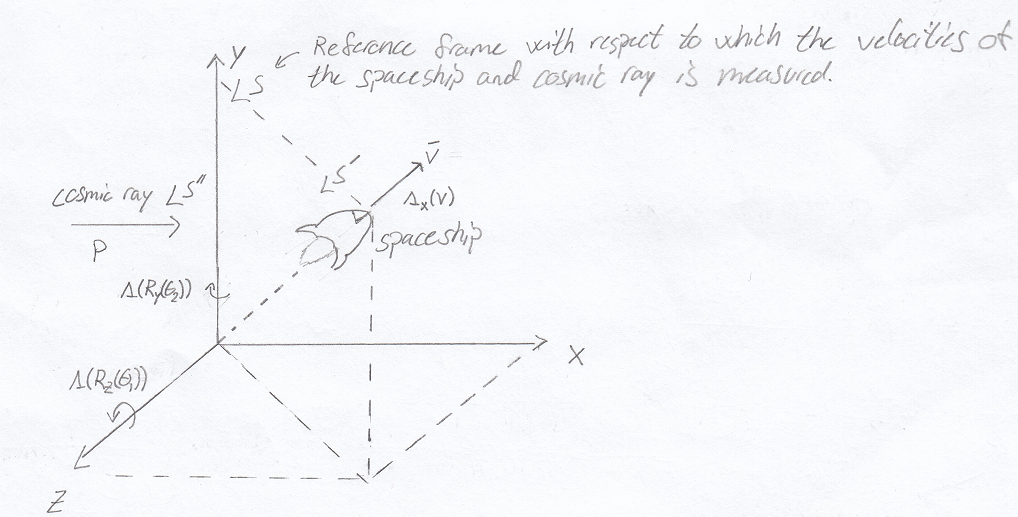
\includegraphics[width=0.6\textwidth]{figures//ss}
		\caption{The scenario with the three reference frames involved.}
		\label{fig:ss}
	\end{figure} 
	\begin{enumerate}
		\item \emph{Find the four velocity, $u$, of the spaceship.}
		
		From $S$
		\begin{equation}
			u=\gamma(v)\begin{bmatrix}
				1 \\
				\vec{v}\\
			\end{bmatrix}=\begin{bmatrix}
				2 \\
				2\vec{v}\\
			\end{bmatrix},
		\end{equation} 
		where $v=|\vec{v}|$.
		
		\item \emph{Find the energy of the cosmic ray in $S'$.}
		
		I know the energy in $S$ from $p$, so I will create a Lorentz transformation to transform $p$ from $S$ to $S'$. To this end I will use a general Lorentz transformation which will consist of two rotations, one boost and the inverse rotations. The idea is to rotate the coordinate-system so it aligns with the velocity of the space-ship, boost so the coordinate system, in rotated form, moved with the spaceships, and lastly rotate the coordinate system back. The result will be a boost of $S$ such that is follows the spaceship, i.e. $S\Rightarrow S'$. First, I will rotate (counter clockwise, i.e. positive angle) around the $z$-axis such that the $\vec{v}$lies in the $zx$ plane. Hereafter I will rotate (clockwise, i.e. negative angle) around the (new, since I have rotated around the $z$-axis) $y$-axis such that the $x$-axis is aligned with $\vec{v}$. Hereafter I will boost along the $x$-axis and rotate back. The Lorentz transformation
		\begin{equation}
			\Lambda_{tot}=\big(\Lambda(R_y(\theta_2))\Lambda(R_z(\theta_1))\big)^{-1}\Lambda_x(\gamma(v))\Lambda(R_y(\theta_2))\Lambda(R_z(\theta_1),
		\end{equation} 
		where
		\begin{equation}
			\Lambda(R_i(\theta_j))=\begin{bmatrix}
				1 & 0 & 0 & 0\\
				0 &   &   &   \\
				0 &   & R_i(\theta_j) & \\
				0 &   &   & \\
			\end{bmatrix}, \quad \Lambda_x(\gamma(v))=\begin{bmatrix}
				\gamma(v)&-v\gamma(v)&0&0\\
				-v\gamma(v)&\gamma(v)&0&0\\
				0&0&1&0\\
				0&0&0&1\\
			\end{bmatrix}.
		\end{equation} 
		Since I know $v$, all I need is the two rotation angles. I find these by considering the criterion for each rotation. After the first rotation the velocity should be in the $zx$-plane, and therefore the transformed velocity should have no $y$-component. Hence, I can find the first rotation angle from
		\begin{equation}
			\begin{split}
				R_z(\theta_1)\vec{v}&\propto\begin{bmatrix}
					cos(\theta_1) & sin(\theta_1) & 0 \\
					-sin(\theta_1) & cos(\theta) & 0 \\
					0 & 0 & 1 \\
				\end{bmatrix}\begin{bmatrix}
					1\\
					1\\
					1\\
				\end{bmatrix}\\
				&=\begin{bmatrix}
					cos(\theta_1)+sin(\theta_1)\\
					sin(\theta_1)-cos(\theta_1)\\
					1\\
				\end{bmatrix}\\
				&= \begin{bmatrix}
					\dots\\
					0\\
					1\\
				\end{bmatrix}.\\
			\end{split}
		\end{equation} 
		In order for the second component of the transformed velocity to vanish $sin(\theta_1)=cos(\theta_1)\Rightarrow \theta_1=\frac{\pi}{4}$. From the second rotation the $x$-axis is to align with $\vec{v}$, so the third component of the transformed velocity is to vanish. Hence, I can find the second rotation angle from
		\begin{equation}
			\begin{split}
				R_y(\theta_2)R_z(\theta_1)\vec{v}&\propto
				\begin{bmatrix}
					cos(\theta_2) & 0 & -sin(\theta_2) \\
					0 & 1 & 0 \\
					sin(\theta_2) & 0 & cos(\theta_2) \\
				\end{bmatrix}\begin{bmatrix}
					\sqrt{2}\\
					0\\
					1\\
				\end{bmatrix}\\
				&=\begin{bmatrix}
					\sqrt{2}cos(\theta_2)-sin(\theta_2)\\
					0\\
					cos(\theta_2)+\sqrt{2}sin(\theta_2)\\
				\end{bmatrix}\\
				&=\begin{bmatrix}
					|\vec{v}|\\
					0\\
					0\\
				\end{bmatrix}.\\
			\end{split}
		\end{equation} 
		In order for the third component of the transformed velocity to vanish; $cos(\theta_2)+\sqrt{2}sin(\theta_2)=0\Rightarrow \theta_2=-35.264 deg$. By using the two rotation angles I can now transform $p$ and find it in $S'$
		\begin{equation}
			p'=\Lambda_{tot}p=\begin{bmatrix}
				301 \\
				296/3\\
				-601/3\\
				-601/3\\
			\end{bmatrix}\cdot 10^{-27}kg.
		\end{equation} 
		Hence, the energy (now in SI units) as seen from $S'$ is $301\cdot 10^{-27}kg\cdot c^2\simeq 2.7\cdot 10^{-8}J$.
		
		\item \emph{Calculate the energy in $S'$ from $-g_{\mu\nu}u^\mu p^\nu$. Why does this work?}
		
		I can also calculate the energy from $-g_{\mu\nu}u^\mu p^\nu$. $-g_{\mu\nu}u^\mu p^\nu$ has all indices contracted and so is a Lorentz scalar. In the rest frame of the spaceship $u^T=\begin{bmatrix}
			1 \\\vec{0}\\
		\end{bmatrix}$ and so it works to pick out the zeroth component of the momentum vector; the energy. So, the quantity is the energy in $S'$ and it is invariant between reference frame. Hence, I can calculate it in $S$ and thereby obtain the energy in $S'$. I find
		\begin{equation}
			\begin{split}
				-g_{\mu\nu}u^\mu p^\nu&=u^0p^0-u^1p^1-u^2p^2-u^3p^3\\
				&=(2\cdot 300-299)\cdot 10^{-27}kg\cdot c^2\\
				&=301\cdot 10^{-27}kg\cdot c^2.
			\end{split}
		\end{equation} 
	\end{enumerate}
\end{example}

\section{The Poincare' group}
The Poincare' group, $ISO(1,3)$, is the group of Lorentz transformations and translations. The Poincare' group encompasses the transformations the physical theories, in the absence of general relativistic effects, should obey, i.e. the physical theory should be invariant under translation, rotation and boosts - Physical theories should be invariant under Poincare' transformations. A generic Poincare' transformation is on the form
\begin{equation}
	x^\mu\Rightarrow {x'}^\mu=\Lambda^{\mu}_{\,\,\, \nu}x^\nu+a^{\mu}.
\end{equation}  
where $a^\mu$ is a constant four vector. From which it is clear that the Poincare' group contains Lorentz transformations and translations. The generators of the Poincare' group are the generators of the Lorentz group, $J_i,K_i$ and the generator of translation in flat space-time (Minkowski space); $p^\mu$. In terms of the generators, the algebra reads
\begin{equation}
	\begin{split}
		&[J_i,J_j]=i\epsilon_{ijk}J_k, \quad [J_i,K_j]=i \epsilon_{ijk}K_k, \quad [K_i,K_j]=-i\epsilon_{ijk}J_k,\\
		&[J_i,p_j]=i\epsilon_{ijk}p_k,\quad [j_i,p_0]=0,\quad [k_i,p_j]=i\delta_{ij}p_0,\quad [k_i,p_0]=-ip_i.
	\end{split}
\end{equation} 


\chapter{Classical field theory}
Field theory is one of the cornerstones of classical physics. The most notable examples of classical fields are the force fields that one encounters in the description of gravitational and electromagnetic phenomena. These fields are caused by the presence of masses and electric charges, respectively. In this chapter I present a framework for classical field theory, which is known as the Lagrangian formulation, alongside a vital theorem relating mathematical symmetries of the Lagrangian to conserved quantities; Noethers theorem.

\section{The Lagrangian formulation of classical field theory}
The framework of classical field theory is the generalization of Lagrangian mechanics to fields. The formulation of Lagrangian mechanics made for classical mechanics was for a finite number of degrees of freedom - fields incorporate an infinite number of degrees of freedom and as such the Lagrangian formalism must be generalized to encompass this scenario. In order to do so the classical Lagrangian is expressed, not as a function of dynamical variables that are functions of time (i.e. $q_i(t)$), but as a function of functions (fields) of space-time\footnote{A function of a function is a functional. Hence, in generalizing the Lagrangian formalism from classical mechanics to classical field theory the Lagrangian goes from being a function to being a functional.}. For a local field theory, a generic Lagrangian ($L$) can be written in terms of the Lagrangian density ($\mathcal{L}$) which is a function of the generic fields ($\phi_a(x)$) and their derivatives ($\partial_\mu\phi_a(x)$),  i.e.
\begin{equation}
	L[\phi_a(x),t]=\int d^3x\mathcal{L}(\phi_a(x),\partial_\mu\phi_a(x)).
\end{equation} 
The Lagrangian density is related to the Hamiltonian density cf.
\begin{equation}
	\mathcal{H}=\sum_a\Pi_a\partial_0\phi_a-\mathcal{L},
	\label{h1}
\end{equation} 
which is in complete analogy with the definition of the Hamiltonian in classical mechanics (see equation \eqref{ham}). In both classical and quantum field theory the theories are formulated in terms of a Lagrangian density because the Lagrangian density is manifestly Lorentz invariant. In general the physical laws are required to be covariant under Poincare' transformations (translations, rotations and boosts). Poincare' covariance is a statement of the familiar principle from classical mechanics; physics should be the same in inertial reference frames. The fields in the action are inherently independent of translations\footnote{The action is invariant under a constant coordinate transformation since this can be absorbed by the integration measure. Take $S=\int d^4x\mathcal{L}(\phi(x),\dots)\Rightarrow S'=\int d^4x\mathcal{L}(\phi(x+a),\dots)=\int d^4y\mathcal{L}(\phi(y),\dots)=S$, where $y=x+a$. Hence, the action is inherently invariant under coordinate translations.}. Hence, the action is only "forced" to be covariant under Lorentz transformations. Since the action is a Lorentz scalar, the Lagrangian density is also the be Lorentz invariant. 

\paragraph{Lorentz covariance:} \emph{A quantity is called Lorentz covariant if the form of the equation does not change under a Lorentz  transformation\index{Lorentz covariance}. An object is Lorentz covariant if it transforms under an irreducible representation of the Lie algebra of the proper, orthochronous Lorentz group.} 

\paragraph{Lorentz invariance:} \emph{A term is Lorentz invariant if it does not change during a proper, orthochronous Lorentz transformation. An object that does not change under proper, orthochronous Lorentz transformations is called a Lorentz scalar.}\newline

To recap; Lorentz covariance is directly derived from the principle that physics should be the same in inertial reference frames. Enforcing Lorentz covariance means that the fields in the Lagrangian density should transform under irreducible representations of the Lie algebra of the proper, orthochronous Lorentz group. In the next section the representations will be derived. Subsequently these representations can be arranged such that the resulting objects are invariant under parity - Which must physical systems are observed to be\footnote{Specifically the spinors are not invariant under parity. Hence, they are arranged in the Dirac spinor which is.}! 

\section{Irreducible (finite) representations of the Lorentz group}
Here the irreducible representations of the Lie algebra of the proper, orthochronous Lorentz group (or equivalently; the irreducible representations of the covering group of the proper, orthochronous Lorentz group) will be determined. The proper, orthochronous Lorentz group is not a simply connected group and as such there is not a one-to-one correspondence between the irreducible representations of the Lie algebra and the the representations of the proper, orthochronous Lorentz group. Instead, there is a one-to-one correspondence between the irreducible representations of the Lie algebra and the covering group of the proper, orthochronous Lorentz group. Hence, when one talks about the irreducible (finite\footnote{"Finite" is used because there is also an infinite dimensional representation of the cover of the proper, orthochronous Lorentz group. These are the matrices responsible for Lorentz transforming $x$. When a field is transformed the field itself is transformed via a finite dimensional representation of the cover of the proper, orthochronous Lorentz group whereas the argument of the field is transformed via the infinite dimensional representation of the cover of the proper, orthochronous Lorentz group. However, how to transform the position four vector in special relativity has already been covered and as such the infinite dimensional representation will not be considered here.}) representations of the Lorentz group, one really talks about the irreducible representations of the covering group (double cover) of the proper, orthochronous Lorentz group. Recall that a covering group is a group which manifold is simply connected. For this reason, groups which have identical Lie algebra must have a manifold that is contained inside the manifold of the covering group. An example is $SU(2)$ and $SO(3)$ (the two groups have the same Lie algebra); the manifold of $SU(2)$ is the unit three sphere whereas the manifold of $SO(3)$ is half the unit three sphere. Since the unit three sphere is simply connected, $SU(2)$ is the simply connected group of this Lie algebra and the manifolds of groups having identical Lie algebra is contained/covered by the manifold of $SU(2)$. The covering group of the proper, orthochronous Lorentz group is $SL(2,\mathbb{C})$; the group of non-degenerate complex matrices with unit determinant. Hence the irreducible representations obtained from the Lie algebra of the proper, orthochronous Lorentz group are the irreducible representations\footnote{Only some of the irreducible representations of the Lie algebra of the proper, orthochronous Lorentz group will be irreducible representations of the proper orthochronous Lorentz group (eg. the spinor representations are not irreducible representations of the proper, orthochronous Lorentz group).} of $SL(2,\mathbb{C})$, and it is these representations that the objects in the Lagrangian density is required to transform under in order to be Lorentz covariant.\newline

To determine the irreducible representations of the covering group of the proper, orthochronous Lorentz group I will begin by considering a field (not necessarily hermitian) that carries a generic Lorentz index, $\phi_a(x)$. Under a Lorentz transformation on the form $x^\mu\Rightarrow {x'}^\mu=\Lambda^\mu_{\,\,\, \nu}x^\nu$ the generic field transforms viz
\begin{equation}
	\phi_a(x^\mu)\Rightarrow \phi'_a({x'}^\mu)=\phi'_a(\Lambda^\mu_{\,\,\, \nu}x^\nu)=D[\Lambda]_{a}^{\,\,\, b}\phi_b(x^\mu),
	\label{pas}
\end{equation} 
where\footnote{The last equality can be intuitively justified by the fact that a scalar field is invariant, i.e. $\phi'(x')=phi(x)$.} $D[\Lambda]_{a}^{\,\,\, b}$ are matrices responsible for the transformation of the field (for a vector field; $D[\Lambda]_{a}^{\,\,\, b}=\Lambda^\mu_{\,\,\, \nu}$). The matrices $D[\Lambda]_{a}^{\,\,\, b}$ form a representation of the covering group of the proper, orthochronous Lorentz group. The proper, orthochronous Lorentz group is a Lie group. Recall from the chapter on group theory: A group is a set of elements $\{g_i\}$ and a rule $g_i\otimes g_j\Rightarrow g_k$ which informs how each pair of elements is multiplied to get a third. A Lie group is a group which is also a differentiable manifold. The manifold of the group can be represented by several representations. A representation is a particular embedding of the group elements into matrices. In this case the transformation matrices, $D[\Lambda]_{a}^{\,\,\, b}$, form a representation of the covering group of the proper, orthochronous Lorentz group. Since $D[\Lambda]_{a}^{\,\,\, b}$ form a representation of the covering group of the proper, orthochronous Lorentz group, they must obey
\begin{equation}
	D[\Lambda_1]D[\Lambda_2]=D[\Lambda_1\Lambda_2],
\end{equation}  
where $D[\Lambda^{-1}]=D[\Lambda]^{-1}$ and $D[I]=I$. The generic transformation $\phi_a(x^\mu)\Rightarrow \phi'_a({x'}^\mu)$ transforms both the fields and coordinates. However, in both classical and quantum field theory \emph{active} coordinate transformations are consider. An active coordinate transformation is a transformation which shifts the field but not the coordinates. That is an active transformation is on the form $\phi_a(x^\mu)\Rightarrow \phi'_a({x}^\mu)$. In order to obtain an active transformation from equation \eqref{pas}, let  $x^\nu\Rightarrow (\Lambda^{-1})^\mu_{\,\,\,\nu}x^\nu$. Hereby
\begin{equation}
	\phi_a(x^\mu)\Rightarrow \phi'_a(x^\mu)=D[\Lambda]_{a}^{\,\,\, b}\phi_b(\Lambda^{-1}x).
	\label{act}
\end{equation} 
Equation \eqref{act} is the form of transformations (active) in both classical and quantum field theory. The covering group of the proper, orthochronous Lorentz group itself is a mathematical object (manifold) independent of any particular representation. To study the group, independent of the representations, a generic element of the group must be expressed in terms of the basis of generators of the group. The covering group of the proper, orthochronous Lorentz group (being a Lie group) has basis generators defined in terms of the deviation (of an infinitesimal, generic element of $SO(3,1)$) from the unity element (see equation \eqref{dj}). That is, the unitary operator must be on the (infinitesimal) form
\begin{equation}
	\Lambda\sim R(dx)=e-idxJ.
\end{equation} 
In the case of the covering group of the proper, orthochronous Lorentz group there are several continuous parameters (analogous to $dx$), eg. the continuous parameters representing the boosts and rotations. These parameters must be collected in some way. To determine the way to perform this (the collection of the parameters), consider an infinitesimal Lorentz transformation parametrized by
\begin{equation}
	\Lambda^\mu_{\,\,\,\nu}=\delta^\mu_{\,\,\,\nu}+\omega^\mu_{\,\,\,\nu}.
	\label{j8}
\end{equation}  
To gain information about $\omega^\mu_{\,\,\,\nu}$ use the parametrization of $\Lambda^\mu_{\,\,\,\nu}$ in the expression for the metric
\begin{equation}
	\begin{split}
		\eta_{\mu\nu}&=\eta_{\alpha\beta}\Lambda^\alpha_{\,\,\,\nu}\Lambda^\beta_{\,\,\,\mu}\\
		&\simeq\eta_{\alpha\beta}(\delta^\alpha_{\,\,\,\nu}+\omega^\alpha_{\,\,\,\nu})(\delta^\beta_{\,\,\,\mu}+\omega^\beta_{\,\,\,\mu})\\
		&=\eta_{\alpha\beta}(\delta^\alpha_{\,\,\,\,\nu}\delta^\beta_{\,\,\,\mu}+\delta^\alpha_{\,\,\,\nu}\omega^\beta_{\,\,\,\mu}+\delta^\beta_{\,\,\,\mu}\omega^\alpha_{\,\,\,\nu}+\omega^\alpha_{\,\,\,\nu}\omega^\beta_{\,\,\,\mu})\\
		&=\eta_{\mu\nu}+\eta_{\nu\beta}\omega^\beta_{\,\,\,\,\mu}+\eta_{\alpha\mu}\omega^\alpha_{\,\,\,\nu}+\omega_{\beta\nu}\omega^\beta_{\,\,\,\mu}\\
		&=\eta_{\mu\nu}+\omega_{\nu\mu}+\omega_{\mu\nu}+\mathcal{O}(\omega^2).
	\end{split}
\end{equation} 
For the above to hold to first order in $\omega$, $\omega$ must be anti-symmetric, i.e. $\omega_{\nu\mu}=-\omega_{\mu\nu}$. As an antisymmetric tensor $\omega_{\mu\nu}$ has six independent parameters, corresponding to $3$ rotational angles and $3$ boosts. To each of the six parameters corresponds a generator (analogous to $J$ in equation \eqref{dj}). These generators are listed in the antisymmetric tensor; $J_{\mu\nu}$. Hence, the usual product $dxJ$ takes the form $\omega^{\mu\nu}J_{\mu\nu}$ in this case. Because of the summation over two anti-symmetric tensors will lead to identical terms, a factor of $\frac{1}{2}$ is included, in the expression for a generic element, in order to account for this "over counting". Thereby a generic element of the covering group of the proper, orthochronous Lorentz group can be written in terms of the generators as
\begin{equation}
	\Lambda=e-\frac{i}{2}\omega^{\mu\nu}J_{\mu\nu}.
	\label{j7}
\end{equation} 
Compounding these infinitesimal transformations to a finite one
\begin{equation}
	\Lambda=e^{-\frac{i}{2}\omega^{\mu\nu}J_{\mu\nu}}.
\end{equation} 
The explicit form of the generators, $J^{\mu\nu}$, depends in the representation. However, since the generators are rank 2 tensors, the generators must transform viz
\begin{equation}
	J^{\mu\nu}\Rightarrow {J'}^{\mu\nu}=\Lambda^{-1}J^{\mu\nu}\Lambda=\Lambda^{\mu}_{\,\,\, \alpha}\Lambda^{\nu}_{\,\,\, \beta}J^{\alpha\beta}.
	\label{j6}
\end{equation} 
Next use equation \eqref{j7} and expand $\Lambda^{-1}J^{\mu\nu}\Lambda$ to first order in $\Omega$
\begin{equation}
	\begin{split}
		\Lambda^{-1}J^{\mu\nu}\Lambda&=\bigg(e-\frac{i}{2}\omega^{\alpha\beta}J_{\alpha\beta}\bigg)J^{\mu\nu}\bigg(e-\frac{i}{2}\omega^{\sigma\rho}J_{\sigma\rho}\bigg)\\
		&=J^{\mu\nu}+\frac{i}{2}\omega_{\alpha\beta}[J^{\mu\nu},J^{\alpha\beta}]+\mathcal{O}(\omega^2).
		\label{j9}
	\end{split}
\end{equation} 
Using equation \eqref{j8} to expand $\Lambda^{\mu}_{\,\,\, \alpha}\Lambda^{\nu}_{\,\,\, \beta}J^{\alpha\beta}$
\begin{equation}
	\begin{split}
		\Lambda^{\mu}_{\,\,\, \alpha}\Lambda^{\nu}_{\,\,\, \beta}J^{\alpha\beta}&=(\delta^\mu_{\,\,\,\nu}+\omega^\mu_{\,\,\,\alpha})(\delta^\mu_{\,\,\,\nu}+\omega^\mu_{\,\,\,\beta})J^{\alpha\beta}\\
		&=J^{\mu\nu}+\omega^\mu_{\,\,\,\alpha}J^{\alpha\nu}+\omega^\nu_{\,\,\,\beta}J^{\mu\beta}+\mathcal{O}(\omega^2)\\
		&=J^{\mu\nu}+\frac{1}{2}\bigg(\omega^\mu_{\,\,\,\alpha}J^{\alpha\nu}+\omega^\mu_{\,\,\,\beta}J^{\beta\nu}+
		\omega^\nu_{\,\,\,\beta}J^{\mu\beta}+\omega^\nu_{\,\,\,\alpha}J^{\mu\alpha}
		\bigg)+\mathcal{O}(\omega^2)\\
		&=J^{\mu\nu}+\frac{1}{2}\bigg(g^{\mu\beta}\omega_{\beta\alpha}J^{\alpha\nu}+g^{\mu\alpha}\omega_{\alpha\beta}J^{\beta\nu}+
		g^{\nu\alpha}\omega_{\alpha\beta}J^{\mu\beta}+g^{\nu\beta}\omega_{\beta\alpha}J^{\mu\alpha}
		\bigg)+\mathcal{O}(\omega^2)\\
		&=J^{\mu\nu}+\frac{1}{2}\omega_{\alpha\beta}\bigg(-g^{\nu\beta}J^{\mu\alpha}-g^{\mu\beta}J^{\alpha\nu}+
		g^{\nu\alpha}J^{\mu\beta}+g^{\mu\alpha}J^{\beta\nu}
		\bigg)+\mathcal{O}(\omega^2).\\
	\end{split}
	\label{j10}
\end{equation} 
Comparing equation \eqref{j9} and \eqref{j10} it is clear that all generators of the Lorentz group should obey the commutator relation
\begin{equation}
	[J^{\mu\nu},J^{\alpha\beta}]=i\bigg(g^{\nu\beta}J^{\mu\alpha}+g^{\mu\beta}J^{\alpha\nu}-
	g^{\nu\alpha}J^{\mu\beta}-g^{\mu\alpha}J^{\beta\nu}\bigg).
\end{equation} 
This is the Lie algebra of $SO(3,1)$. In order to analyse the representations of the covering group of the proper, orthochronous proper, orthochronous Lorentz group it is convenient to introduce the rotation generators, $J^{i}$, and the boost generators, $K^{j}$, viz
\begin{equation}
	J^i\equiv\frac{1}{2}\epsilon^{ijk}J^{jk}, \quad K^i\equiv J^{i0}.
\end{equation} 
In terms of these definitions, the Lie algebra is given by
\begin{equation}
	[J^i,J^j]=i\epsilon^{ijk}J^{k}, \quad [J^i,K^j]=i\epsilon^{ijk}K^{k}, \quad [K^i,K^j]=-i\epsilon^{ijk}J^{k}.
\end{equation} 
From the above it is clear $J^i$ obey the Lie algebra of $SU(2)$, however the $K^i$ does not. To simplify the Lie algebra further, make another redefinition viz
\begin{equation}
	M^i\equiv \frac{1}{2}(J^i+iK^i), \quad N^i\equiv \frac{1}{2}(J^i-iK^i)=(M^i)^\dagger.
\end{equation} 
The redefined generators obey the commutator relations given by
\begin{equation}
	[M^i,M^j]=i\epsilon^{ijk}M^{k}, \quad [N^i,N^j]=i\epsilon^{ijk}N^{k}, \quad [M^i,N^j]=0.
	\label{gen}
\end{equation} 
These are precisely the commutator relations for the Lie algebra of $SU(2)$. It is therefore clear that the Lie algebra of the proper, orthochronous Lorentz groups consists of two copies of $SU(2)$, i.e. $SU(2)\otimes SU(2)$. This is good news since the irreducible representations the Lie algebra of $SU(2)$ are well determined~\citep{Schwichtenberg2015}. Because the Lorentz group can be described as a $SU(2)\otimes SU(2)$, and the $SU(2)$ Lie algebra is the algebra of angular momentum, a particular representation can be specified by two quantum numbers of angular momentum; $j,j'$\footnote{To keep notation it would have to be $n,m$ but $j,j'$ is conventionally taken.}. In group theoretical terms, the representations are specified by the eigenvalues of Casimir operators. A Casimir operators is an operator built from generators that commute with all generators of the group. The eigenvalue of the Casimir operator has a constant value for each representation and is hence suited for labelling the representation. The Casimir operator of $SU(2)$ which eigenvalues label the representations is $J^2$. The eigenvalues are denoted by $j$. Hence, since the covering group of the proper, orthochronous Lorentz group is $SU(2)\otimes SU(2)$, this groups is labelled by the eigenvalues of two Casimir operators; $J_1^2, J_2^2$; $(j_1,j_2)$ and has $(2j+1)(2j'+1)$ degrees of freedom,  i.e.
\begin{equation}
	(j,j'), \quad \text{where: } j,j'=0,\frac{1}{2},1,....
\end{equation} 
The regular rotation generators are given by $\vec{J}=\vec{M}+\vec{N}$, and each representation contains particles of spin $J=j+j', j+j'-1,\dots |j-j'|$. This leads to the possible representations and the associated angular momentum:\newline
\begin{center}
	\begin{tabular}{ |l|l|l| }
		\hline
		Notation & Representation & Angular momentum \\ \hline
		Scalar & $\big(0,0\big)$ & $J=0$ \\
		Left handed spinor & $\big(\frac{1}{2},0\big)$ & $J=\frac{1}{2}$ \\
		Right handed spinor & $\big(0,\frac{1}{2}\big)$ & $J=\frac{1}{2}$ \\
		Vector & $\big(\frac{1}{2},\frac{1}{2}\big)$ & $J=\frac{1}{2},0$ \\
		\hline
	\end{tabular}
\end{center}
where the most used representations (scalar, spinor, vector,... ) have been listed. Hence, fields which transform under the above representations are allowed in Lagrangian densities that are to describe physical systems. 
\begin{example}
	The lowest order representation, $(0,0)$, called the scalar representation, is quite  trivial because the vector space is one dimensional for both copies of the Lie algebra of $SU(2)$. The generators must therefore be $1\times 1$ matrices. The only $1\times 1$ matrices that satisfy the commutator relations of the generators, i.e. equation \eqref{gen} are trivially $0$. Hereby
	\begin{equation}
		J_{\mu\nu}=0\Rightarrow \Lambda=e.
	\end{equation} 
	Therefore the scalar representation acts on objects that do not change under Lorentz transformations. Therefore, the scalar field transforms viz
	\begin{equation}
		\phi(x)\Rightarrow \phi'(x)=\phi(\Lambda^{-1}x).
	\end{equation} 
\end{example}

\begin{example}
	The $(\frac{1}{2},0)$ representation is called the left handed spinor representation. The left-handed spinor field transforms viz
	\begin{equation}
		\psi_a(x)\Rightarrow \psi'_a(x)=L[\Lambda]_a^{\,\,\, b}\psi_b(\Lambda^{-1}x),
	\end{equation} 
	where for an infinitesimal transformation
	\begin{equation}
		L[\Lambda]_a^{\,\,\, b}=\delta_a^{\,\,\, b}-\frac{i}{2}\omega^{\mu\nu}(S^{(L)}_{\mu\nu})_a^{\,\,\, b},
	\end{equation} 
	where $(S_{(L)}^{\mu\nu})_a^{\,\,\, b}=-(S_{(L)}^{\nu\mu})_a^{\,\,\, b}$ are the representation matrices which must obey the same algebra as the generators of the Lorentz group (i.e. the commutator relation of $J^{\mu\nu}$). Using the same $\omega^{\mu\nu}$ in $L[\Lambda]$ as in $\Lambda(\omega)$ ensures that $x,\psi$ are subject to the same Lorentz transformation.	
\end{example}
\begin{example}
	The $(0,\frac{1}{2})$ representation is called the right handed spinor representation. Taking the hermitian conjugate swaps the $SU(2)$ Lie algebras of the Lorentz group. Therefore, the hermitian conjugate of a left-handed spinor field should be a right-handed spinor field. Indices of right handed spinors are denoted, following the notation of \citet{Srednicki2027}, with a dot viz\footnote{This notation is called the Van der Waerden Notation~\citep{Schwichtenberg2015}.}
	\begin{equation}
		[\psi_a(x)]^\dagger=\psi_{\dot{a}}^\dagger(x).
	\end{equation} 
	Taking the hermitian conjugate of the transformation of a left-handed spinor
	\begin{equation}
		\psi^\dagger_{\dot{a}}(x)\Rightarrow {\psi'}^\dagger_a(x)=R[\Lambda]_{\dot{a}}^{\,\,\, \dot{b}}\psi^\dagger_{\dot{b}}(\Lambda^{-1}x),
	\end{equation} 
	where for an infinitesimal transformation
	\begin{equation}
		R[\Lambda]_{\dot{a}}^{\,\,\, \dot{b}}=\delta_{\dot{a}}^{\,\,\, \dot{b}}-\frac{i}{2}\omega^{\mu\nu}(S^{(R)}_{\mu\nu})_{\dot{a}}^{\,\,\, \dot{b}}.
	\end{equation} 
\end{example}
\begin{example}
	The $(\frac{1}{2},\frac{1}{2})$ representation is called the vector representation. This representation is the one familiar form special relativity\footnote{The generators can be found in~\citet{Peskin1995}[p. 39].}. A vector field transforms viz
	\begin{equation}
		A^{\mu}(x)\Rightarrow {A'}^{\mu}(x)=\Lambda^\mu_{\,\,\,\nu}A^\nu(\Lambda^{-1}x).
	\end{equation} 
\end{example}

\subsection{Construction a Lagrangian density}
At this point it has been established that in field theory the primary content of the Lagrangian density is fields. The allowed fields in the Lagrangian must transform under an irreducible representation of the cover group of the proper, orthochronous Lorentz group. whereas the scalar and vector fields are invariant under parity, the spinor fields are not. The easiest thing to do to build a parity invariant quantity from the spinors is to write them into a Dirac field. The Dirac field\index{Dirac field} is defined viz
\begin{equation}
	\Psi_D(x)=\psi_L(x)\oplus\psi_R(x)\doteq\begin{bmatrix}
		\psi_L(x)\\
		\psi_R(x)\\
	\end{bmatrix},
\end{equation} 
where $\psi_{L,R}(x)$ are left handed and right handed spinor fields, respectively. Usually only Dirac fields are considered, and as such the subscript $D$ is omitted. The left handed spinor transforms via $L[\Lambda]$ whereas the right handed spinor transforms via $R[\Lambda]$. Hence, the transformation of the Dirac field can be written viz
\begin{equation}
	\Lambda_D=\begin{bmatrix}
		L[\Lambda] & 0 \\
		0 & R[\Lambda]\\
	\end{bmatrix}.
\end{equation} 
That is
\begin{equation}
	\Psi(x)\Rightarrow \Psi'(x')=\Lambda_D\Psi(\Lambda^{-1}x).
\end{equation} 
By introducing the Dirac field, the fields available to build Lagrangians form are\footnote{There are higher representations available but these are the most fundamental and suffice to describe all known particles.}
\begin{equation}
	\begin{split}
		\text{Available fields:} \quad \{&\text{scalar } (\phi(x)), \quad \text{Dirac} (\Psi(x)), \quad \text{vector} (A^\mu(x))\dots\}.
	\end{split}
\end{equation} 
From these fields, Lorentz scalars can be constructed. In order for the Lagrangian density to be Lorentz invariant, it must be a Lorentz scalar. Hence, the terms in the Lagrangian must be Lorentz scalars, i.e.
\begin{equation}
	\mathcal{L}=\sum_i (\text{Lorentz scalars})_i.
\end{equation} 
Lorentz scalars terms that transform like a scalar under a Lorentz transformation.
\begin{example}
	An example of a Lorentz scalar is $\bar{\psi}(x)\psi(x)$, where both fields are Dirac spinors. $\bar{\psi}(x)\psi(x)$ transforms viz
	\begin{equation}
		\begin{split}
			\bar{\psi}(x)\psi(x)\Rightarrow \psi^\dagger(\Lambda ^{-1}x) \Lambda_D^\dagger\gamma^0\Lambda_D\psi(\Lambda^{-1}x)&=\psi^\dagger(\Lambda ^{-1}x) \gamma^0\psi(\Lambda^{-1}x)\\
			&=\bar{\psi}(\Lambda ^{-1}x)\psi(\Lambda^{-1}x).
		\end{split}
	\end{equation} 
\end{example}
In general, the terms of Lagrangian densities are arranged into two categories; kinetic terms and potential terms. In general, the kinetic terms contain the derivative of the field. The potential terms are more complicated to make broad statements about. For a spin half field, which most fields are, all potential terms (they must be Lorentz scalars) can be constructed from what is called bilinears. In relation to the standard model i quantum field theory all known particles of spin half are described by Dirac fields. The Dirac bilinears are on the form
\begin{equation}
	\text{Form of Dirac field bilinears: }\bar{\psi}(x)\Gamma\psi(x),
\end{equation} 
where $\Gamma$ is a $4\times 4$ constant matrix. The possible $\Gamma's$ are categorized into groups according to how they transform under the Lorentz group
\begin{equation}
	\begin{split}
		& \text{Scalar: } \,\,\qquad\qquad \Gamma=I,\\
		& \text{Vector: } \,\qquad\qquad \Gamma=\gamma^\mu,\\
		& \text{Tensor: } \,\qquad\qquad \Gamma=\sigma^{\mu\nu}=\frac{i}{2}[\gamma^\mu,\gamma^\nu],\\
		& \text{Pseudo-vector: } \quad \Gamma=\gamma^\mu\gamma^5,\\
		& \text{Pseudo-scalar: }\, \quad \Gamma=i\gamma^5,\\
	\end{split}
	\label{bilinears}
\end{equation} 
where the $i$'s are added to make the terms Hermitian. The terms involving "pseudo" transforms as vectors and scalars, respectively, under the continuous Lorentz group (proper, orthochronous transformations), but acquire a sign change under parity transformation. The non-scalar terms contain uncontracted Lorentz indices and as such they must be contracted with therms containing corresponding Lorentz indices in order to transform as a scalar under the Lorentz group. 
\begin{example}
	One common Lagrangian density is the Klein-Gordon (KG) Lagrangian density. The KG Lagrangian density comes in two versions; for a complex scalar field and for a real scalar field. Here the case of a complex scalar field will be considered. The KG equation consists of the simplest kinetic and potential terms
	\begin{equation}
		\text{KG:}\quad \mathcal{L}=(\partial_\mu \phi)^*\partial^\mu\phi-m^2\phi^*\phi.
	\end{equation} 
\end{example}
\begin{example}
	\index{Klein-Gordon equation}
	\index{Gauge invariance}
	\emph{Consider the following Lagrangian density (Klein-Gordon Lagrangian density)}
	\begin{equation}
		\mathcal{L}=(D_\mu\phi)^*D^\mu\phi-m^2\phi^*\phi,
		\label{KG}
	\end{equation} 
	\emph{where $D_\mu=\partial_\mu-igA_\mu$. Show that the KG Lagrangian density is invariant under the Gauge transformation given by}
	\begin{equation}
		\phi\Rightarrow \phi e^{i\alpha(x)} \qquad \mbox{and} \qquad A_\mu\Rightarrow A_\mu+\partial_\mu\Lambda(x).
	\end{equation} 
	\emph{Find also a relation between $\alpha(x)$ and $\Lambda(x)$.}\newline
	
	Begin by inserting the Gauge transformation and write the expression out
	\begin{equation}
		\begin{split}
			\mathcal{L}&=\underbrace{\bigg(\partial_\mu+ig(A_\mu+\partial_\mu\Lambda(x))\bigg)\phi^* e^{-i\alpha(x)}\bigg(\partial^\mu-ig(A^\mu+\partial^\mu\Lambda(x))\bigg)\phi e^{i\alpha(x)}}_{\mathcal{L}_1}\\
			&\qquad-\underbrace{m^2\phi^* e^{-i\alpha(x)}\phi e^{i\alpha(x)}}_{\mathcal{L}_2}.\\
		\end{split}
		\label{eq18}
	\end{equation} 
	In the last term ($\mathcal{L}_2$) the exponentials cancel each other out and the term reduces to the one before the transformation. Therefore it comes down to the first term
	\begin{equation}
		\begin{split}
			\mathcal{L}_1&=\bigg(\partial_\mu+ig(A_\mu+\partial_\mu\Lambda(x))\bigg)\phi^* e^{-i\alpha(x)}\bigg(\partial^\mu-ig(A^\mu+\partial^\mu\Lambda(x))\bigg)\phi e^{i\alpha(x)}\\
			&=\bigg(e^{-i\alpha(x)}\partial_\mu(\phi^*)-i\phi^*e^{-i\alpha(x)}\partial_\mu(\alpha(x))+igA_\mu\phi^*e^{-i\alpha(x)}+ig\partial_\mu(\Lambda(x))\phi^* e^{-i\alpha(x)}\bigg)\\
			&\qquad\cdot \bigg(e^{i\alpha(x)}\partial^\mu(\phi)+i\phi e^{i\alpha(x)}\partial^\mu(\alpha(x))-igA^\mu\phi e^{i\alpha(x)}-ig\partial^\mu(\Lambda(x))\phi e^{i\alpha(x)}\bigg).\\
		\end{split}
		\label{mother}
	\end{equation} 
	Pull out the exponentials from each term and let them cancel
	\begin{equation}
		\begin{split}
			\mathcal{L}_1&=\bigg(\partial_\mu\phi^*-i\phi^*\partial_\mu\alpha(x)+igA_\mu\phi^*+ig\partial_\mu\Lambda(x)\phi^* \bigg) \bigg(\partial^\mu\phi+i\phi \partial^\mu\alpha(x)-igA^\mu\phi -ig\partial^\mu\Lambda(x)\phi \bigg)\\
			&=\bigg(D_\mu\phi^*-i\phi^*\partial_\mu\alpha(x)+ig\partial_\mu\Lambda(x)\phi^* \bigg) \bigg(D^\mu\phi+i\phi \partial^\mu\alpha(x) -ig\partial^\mu\Lambda(x)\phi \bigg).
		\end{split}
	\end{equation} 
	If the last two terms in each parenthesis cancel the Lagrangian reduces to the Lagrangian before transformation and hence the Lagrangian is invariant to the gauge transformation. That is gauge invariance requires
	\begin{equation}
		-i\phi^*\partial_\mu\alpha(x)+ig\partial_\mu\Lambda(x)\phi^* =0,
	\end{equation} 
	\begin{equation}
		i\phi \partial^\mu\alpha(x)-ig\partial^\mu\Lambda(x)\phi =0.
	\end{equation} 
	Both equations are satisfied if $\alpha(x)=g\Lambda(x)$. Which when inserted in equation \ref{eq18} reduces it to 
\end{example}
\begin{example}
	The perhaps most used Lagrangian density in both classical and quantum field theory is the Dirac Lagrangian density. The Dirac Lagrangian density is a function of the Dirac field (made up of spinor fields). It contains a slightly more complicated kinetic term alongside the simplest potential term
	\begin{equation}
		\text{Dirac:}\quad \mathcal{L}=\bar{\psi}(i\gamma^\mu \partial_\mu-m)\psi.
	\end{equation}  
\end{example}
\begin{example}
	\index{Lagrangian in SR}
	\index{Lagrangian on covariant form}
	\index{Hamiltonian in SR}
	\index{Hamiltonian on covariant form}
	\index{Tensor notation in SR}
	\emph{Determine the Hamiltonian density given the Lagrangian density}
	\begin{equation}
		\mathcal{L}=-\frac{1}{4\mu_0}F^{\mu\nu}F_{\mu\nu}-A_{\mu}J^{\mu}.
	\end{equation} 
	Use that the Hamiltonian is found by performing a Legendre transformation of the Lagrangian. From equation \eqref{h1}
	\begin{equation}
		\mathcal{H}=\frac{\partial \mathcal{L}}{\partial(\partial_0 A_\alpha)}\partial_{0}A_\alpha-\mathcal{L}.
	\end{equation} 
	In order to evaluate the above the Lagrangian density must be expressed entirely in terms of $A_\mu$ (with the index down). by doing so and subsequently taking the derivative
	\begin{equation}
		\begin{split}
			\frac{\partial \mathcal{L}}{\partial(\partial_\beta A_\alpha)}&=\frac{\partial}{\partial(\partial_\beta A_\alpha)}\bigg(-\frac{1}{4\mu_0}F^{\mu\nu}F_{\mu\nu}-A_{\mu}J^{\mu}\bigg)=-\frac{1}{4\mu_0}\frac{\partial}{\partial(\partial_\beta A_\alpha)}\bigg(F^{\mu\nu}F_{\mu\nu}\bigg)\\
			&=-\frac{1}{4\mu_0}\frac{\partial}{\partial(\partial_\beta A_\alpha)}\bigg((\partial^\mu A^\nu-\partial^\nu A^\mu)(\partial_\mu A_\nu-\partial_\nu A_\mu)\bigg)\\
			&=-\frac{1}{4\mu_0}\frac{\partial}{\partial(\partial_\beta A_\alpha)}\bigg(\partial^\mu A^\nu\partial_\mu A_\nu-\partial^\mu A^\nu\partial_\nu A_\mu-\partial^\nu A^\mu\partial_\mu A_\nu+\partial^\nu A^\mu\partial_\nu A_\mu\bigg)\\
			&=-\frac{1}{2\mu_0}\frac{\partial}{\partial(\partial_\beta A_\alpha)}\bigg(\partial^\mu A^\nu\partial_\mu A_\nu-\partial^\mu A^\nu\partial_\nu A_\mu\bigg)\\
			&=-\frac{g^{\mu\lambda}g^{\nu\sigma}}{2\mu_0}\frac{\partial}{\partial(\partial_\beta A_\alpha)}\bigg(\partial_\lambda A_\sigma\partial_\mu A_\nu-\partial_\lambda A_\sigma\partial_\nu A_\mu\bigg)\\
			&=-\frac{g^{\mu\lambda}g^{\nu\sigma}}{2\mu_0}\bigg(\delta_\lambda^\beta\delta_\sigma^\alpha \partial_\mu A_\nu+\delta_\mu^\beta\delta_\nu^\alpha\partial_\lambda A_\sigma-\delta_\lambda^\beta\delta_\sigma^\alpha\partial_\nu A_\mu-\delta_\nu^\beta\delta_\mu^\alpha\partial_\lambda A_\sigma\bigg)\\
			&=-\frac{1}{2\mu_0}\bigg(g^{\mu\beta}g^{\nu\alpha}\partial_\mu A_\nu+g^{\beta\lambda}g^{\alpha\sigma}\partial_\lambda A_\sigma-g^{\mu\beta}g^{\nu\alpha}\partial_\nu A_\mu-g^{\beta\lambda}g^{\alpha\sigma}\partial_\lambda A_\sigma\bigg)\\
			&=-\frac{1}{2\mu_0}\bigg(g^{\mu\beta}g^{\nu\alpha}(\partial_\mu A_\nu-\partial_\nu A_\mu)+g^{\beta\lambda}g^{\alpha\sigma}(\partial_\lambda A_\sigma-\partial_\lambda A_\sigma)\bigg)\\
			&=-\frac{1}{2\mu_0}\bigg(g^{\mu\beta}g^{\nu\alpha}F_{\mu\nu}+g^{\beta\lambda}g^{\alpha\sigma}F_{\lambda\sigma}\bigg)=-\frac{F^{\beta\alpha}}{\mu_0}.\\
		\end{split}
	\end{equation} 
	Using this in the expression for the Hamiltonian density
	\begin{equation}
		\mathcal{H}=\frac{1}{4\mu_0}F^{\mu\nu}F_{\mu\nu}+A_{\mu}J^{\mu}-\frac{F^{0\alpha}}{\mu_0}\partial_{0}A_\alpha.
	\end{equation} 
\end{example}

\subsection{The Euler-Lagrange equation in field theory}
To obtain the equations of motion from the Lagrangian density in field theory a generalized version of the Euler-Lagrange equation from classical mechanics can be used. The generalized Euler-Lagrange equation is found by, just as in classical mechanics, varying the action. In field theory the action is given as follows (see equation \eqref{action} to compare with classical mechanics) 
\begin{equation}
	S[\phi_a(x)]=\int d^4x\mathcal{L}(\phi_a(x),\partial_\mu\phi_a(x)).
\end{equation} 
The action is a functional of the fields. Consider now the change in the action when the fields are changed (leaving the coordinates alone), i.e. consider the change in the action under
\begin{equation}
	\delta_0 \phi_a(x)=\phi'_a(x)-\phi_a(x),
\end{equation} 
where the subscript $0$ indicates that the space-time coordinate is fixed during the variation. The variation in the action
\begin{equation}
	\begin{split}
		\delta_0 S[\phi_a(x)]&=\int d^4x\delta_0\mathcal{L}(\phi_a(x),\partial_\mu\phi_a(x))\\
		&=\int d^4x\bigg(\frac{\partial \mathcal{L}(\phi_a(x),\partial_\mu\phi_a(x))}{\partial \phi_a(x)}\delta_0 \phi_a(x)+\frac{\partial \mathcal{L}(\phi_a(x),\partial_\mu\phi_a(x))}{\partial (\partial_\mu\phi_a(x))}\delta_0 (\partial_\mu\phi_a(x))\bigg)\\
		&=\int d^4x\bigg(\frac{\partial \mathcal{L}(\phi_a(x),\partial_\mu\phi_a(x))}{\partial \phi_a(x)}-\partial_\mu \frac{\partial \mathcal{L}(\phi_a(x),\partial_\mu\phi_a(x))}{\partial (\partial_\mu\phi_a(x))}\bigg)\delta_0 \phi_a(x)\\
		&=0,\\
	\end{split}
	\label{s1}
\end{equation} 
where it has been used that $\delta_0$ and $\partial_\mu$ commute, partial integration and that the boundary term vanishes\footnote{The boundary terms vanish because the endpoints of the path is fixed - just like in the case of classical mechanics.}. For equation \eqref{s1} to be valid for every $\delta_0 \phi_a(x)$
\begin{equation}
	\frac{\partial \mathcal{L}}{\partial \phi_a}-\partial_\mu\frac{\partial \mathcal{L}}{\partial (\partial_\mu\phi_a)}=0.
	\label{EL1}
\end{equation} 
This is the Euler-Lagrange equation generalized to field theory. From equation \eqref{EL1}, and the specified Lagrangian density, the EOM for the fields can be determined. 
\begin{example}
	\index{Dirac equation}
	\emph{Consider the Dirac equation}
	\begin{equation}
		(i\gamma^{\mu}\partial_\mu-m)\psi=0.
	\end{equation} 
	\emph{By defining $\bar{\psi}=\psi^\dagger\gamma^{(0)}$ the Dirac equation can be derived from the Lagrangian density}
	\begin{equation}
		L=\bar{\psi}(i\gamma^{\mu}\partial_\mu-m)\psi.
	\end{equation} 
	
	\begin{enumerate}
		\item \emph{Treating $\bar{\psi}$ and $\psi$ as independent fields, show that the Lagrangian results in the Dirac equation.}\newline
		
		The equation of motion, which the Dirac equation is, can be found by using the Lagrangian density in the Euler-Lagrange equation. Since there are two field there are two equations of motion. These equations of motion are equivalent in this case. Consider the equation of motion obtained from $\bar{\psi}$
		\begin{equation}
			\frac{\partial L}{\partial \bar{\psi}}-\partial_\mu\frac{\partial L }{\partial (\partial_\mu\bar{\psi})}=0\Rightarrow (i\gamma^{\mu}\partial_\mu-m)\psi=0.
		\end{equation} 
		Since the Lagrangian does not depend on the derivative of the $\bar{\psi}$-field. 
		
		\item \emph{Find the conjugate momentum densities $\pi_{\psi}$ and $\pi_{\bar{\psi}}$ and use these to construct the Hamiltonian density.}\newline
		
		The conjugate momenta is given by
		\begin{equation}
			\frac{\partial L }{\partial (\partial_0\phi_i)}=\pi_{i}.
		\end{equation} 
		If the field is a vector, so is the conjugate momentum. Immediately it is clear that the momentum conjugate to $\bar{\psi}$ is zero. For the $\psi$-field
		\begin{equation}
			\pi=\frac{\partial L }{\partial (\partial_0\psi)}=\bar{\psi}i\gamma^{0}\partial_0\psi=i\psi^\dagger \gamma^{0}\gamma^{0}=i\psi^\dagger I_{4\times 4}=i\psi^\dagger.
		\end{equation} 
		The Hamiltonian density operator
		\begin{equation}
			H=\partial_t\psi\cdot\pi-L=i\psi^\dagger\partial_t\psi -\bar{\psi}(i\gamma^{\mu}\partial_\mu-m)\psi.
		\end{equation} 
	\end{enumerate}
\end{example}
\begin{example}
	\emph{Derive Diracs equation for a classical field in the way Dirac did it.}\newline
	
	To derive the Dirac equation the basic idea used by Dirac was to factorize the relativistic expression for the energy ($E^2=\vec{p}\,^2+m^2$) into the form
	\begin{equation}
		\begin{split}
			H^2&=(\vec{\alpha}\cdot\vec{p}+\beta m)^2\\
			&=(\sum_{i} \alpha^{i}p_i+\beta m)(\sum_{j} \alpha^{j}p_j+ \beta m)\\
			&=\sum_{i,j} \alpha^{i}p_i \alpha^{j}p_j+\sum_{i} \alpha^{i}p_i\beta m+\sum_{j} \beta m \alpha^{j}p_j+ \beta^2m^2,
		\end{split}
		\label{bla5}
	\end{equation} 	
	where $\vec{\alpha}$ is a three component vector in which each component is a $4\times4$ matrix and $\beta$ is a $4\times4$ matrix. Because $H$ must have real eigenvalues (it is hermitian), and $p_i$ is hermitian, it follows that $\alpha^{i}$ and $\beta$ must be hermitian matrices\footnote{A hermitian matrix satisfies $A=(A^T)^*$.}. Note that $\vec{\alpha}$ and $\beta$ cannot simply be number if the equation is to have rotational invariance. By assuming that $[\alpha^{i},p_j]=0$, $[p_i,\beta]=0$ and utilizing the Einstein summation notation
	\begin{equation}
		\begin{split}
			E^2&=\alpha^{i}\alpha^{j}p_ip_j+(\alpha^{i}\beta+\beta\alpha^{i})p_im+\beta^2m^2\\
			&=\frac{1}{2}(\alpha^{i}\alpha^{j}+\alpha^{j}\alpha^{i})p_ip_j+(\alpha^{i}\beta+\beta\alpha^{i})p_im+\beta^2m^2.\\
		\end{split}
	\end{equation} 	
	This should correspond to $E^2=\vec{p}\,^2+m^2$. Therefore the prefactor in the term with $p_ip_j$ should equal $2\delta_{ij}$. Also the prefactor of the $p_im$-term should vanish and $\beta^2=I_{4\times 4}$. Explicitly written
	\begin{equation}
		\frac{1}{2}\sum_{i,j}(\alpha^{i}\alpha^{j}+\alpha^{j}\alpha^{i})=\delta^{ij}\Rightarrow \alpha^{i}\alpha^{j}+\alpha^{j}\alpha^{i}=\{\alpha^{i},\alpha^{j}\}=2I_{4\times 4},
	\end{equation} 
	\begin{equation}
		\alpha^{i}\beta+\beta\alpha^{i}=0\Rightarrow \{\alpha^{i},\beta\}=0,
		\label{bla6}
	\end{equation} 
	\begin{equation}
		\beta^2m^2=I_{4\times 4}m^2\Rightarrow \beta^2=I_{4\times 4}.
	\end{equation} 
	The specific form of the $\alpha$-and $\beta$-matrices can be found by taking the $\beta$-matrix to be diagonal. It must also be traceless, so therefore the diagonal is of an equal number of "ones" with different sign. That is
	\begin{equation}
		\beta=\begin{bmatrix}
			I_{2\times 2} & 0\\
			0 & -I_{2\times 2}  \\
		\end{bmatrix}.
	\end{equation} 
	From this $\beta$-matrix the $\alpha$-matrices can be found by expressing it (the $\alpha$-matrix) sa a general, hermitian matrix. Hereafter the general hermitian matrix can be made to obey equation \ref{bla6} in order to limit the components of the general matrix. It will be found that the remaining components, the off diagonal-ones in block form, must obey an anti-commutator relation to the Pauli matrices ($\{\sigma^{i},\sigma^{j}\}=2I_{2\times 2}$). Therefore the $\alpha$-matrices can be expressed in terms of the Pauli matrices.
	\begin{equation}
		\alpha^{i}=\begin{bmatrix}
			0 & \sigma^{i}\\
			\sigma^{i} & 0 \\
		\end{bmatrix}.
	\end{equation} 
	This set of $\alpha$- and $\beta$-matrices satisfy the factorization condition given in equation \ref{bla5}. This Hamiltonian is used in Schroedingers equation. However, in order to fulfill the dimensional requirements the wave-function must now be a $4\times1$  matrix. By insertion into the SE
	\begin{equation}
		i\partial_t\psi=-i\alpha^{i}\nabla_i\psi-m\beta\psi.
	\end{equation}  
	By acting with $\beta$ from the left
	\begin{equation}
		i\partial_t(\beta\psi)=-i\beta\alpha^{i}\nabla_i\psi-m\beta^2\psi.
	\end{equation}  
	Next up use that $\beta^2=I_{4\times 4}$ and define now the $\gamma$-matrices
	\begin{equation}
		\gamma^{i}=\beta\alpha^{i}=\begin{bmatrix}
			0 & \sigma^{i}\\
			-\sigma^{i} & 0\\
		\end{bmatrix} \qquad \mbox{and} \qquad \gamma^{0}=\beta=\begin{bmatrix}
			I & 0\\
			0 & -I\\
		\end{bmatrix}.
	\end{equation} 
	From these definitions the Schroedinger equation with the modified Hamiltonian can be written as\footnote{To be explicit; without Einstein notation and in SI units: $\sum_{\mu=0}^{3}(i\hbar\gamma^{\mu}\partial_\mu-mc)\psi=0$.}
	\begin{equation}
		(i\gamma^{\mu}\partial_\mu-m)\psi=0.
	\end{equation} 
\end{example}

\section{Noethers theorem}
The time has come for one of the most important theorems in modern physics; Noethers theorem. Noethers theorem can be stated as follows\index{Noethers theorem, classical field theory}
\paragraph{Noethers theorem:} \emph{If the Lagrangian density for a physical system is not affected by a continuous change (transformation) in the coordinate system used to describe it, then there will be a corresponding conservation law.}\newline

Noethers theorem has a special place in most theoretical physicists hearts. The reason for this is that it connects a mathematical symmetry of a Lagrangian density with a physical property (symmetry) of a physical system. For example, most physical systems are invariant with respect to a space-time translation. The Lagrangian density for such systems must have the same symmetry (the Lagrangian density is to describe the physical system after all, so it better have the same symmetries). Corresponding to the symmetry must be a conserved quantity. In the case of a Lagrangian density with a space-time symmetry (invariant with respect to translations in space and time), there are two conserved quantities; time $\Rightarrow$ energy and space $\Rightarrow$ momentum. Likewise other conserved quantities can be connected to the physical layout of the system. The theorem therefore invites an interpretation of conservation laws as a result of the physical layout of a system. This is a profound result and allows physicists to search for conserved quantities by searching for symmetries of the Lagrangian density. Conversely, if one is to construct a Lagrangian density for a system with a given set of symmetries, it is now clear how these are implemented (via making the Lagrangian density invariant under transformations). \newline  
Corresponding to the conserved quantity is a current with vanishing divergence. This can be determined from the symmetry by investigating the variation in the action carefully. It goes as follows; consider a Lagrangian density that is invariant under the generic transformations
\begin{equation}
	x^\mu\Rightarrow {x'}^{\mu}=x^\mu+\delta x^\mu, \quad \phi_a(x)\Rightarrow \phi'_a(x')=\phi_a(x)+\delta \phi_a(x).
\end{equation} 
Note that, in contrast to the derivation of the Euler-Lagrange equation for field theory, now the coordinates are varied as well as the fields. Take the transformations to be parameterized by some infinitesimal parameter, $\varepsilon^\nu$, such that
\begin{equation}
	{x'}^\mu|_{\varepsilon^\nu=0}=x^\mu, \quad \phi'_i(x')|_{\varepsilon^\nu=0}=\phi_i(x).
\end{equation} 
The change in the action is given by
\begin{equation}
	\begin{split}
		\delta S[\phi_a(x)]&= \int_{\Omega'} d^4x' \mathcal{L}(\partial_\mu\phi_a'(x'),\phi_a'(x'))-\int_{\Omega}d^4x\mathcal{L}(\partial_\mu\phi_a(x),\phi_a(x))=0\\
	\end{split},
	\label{k}
\end{equation} 
where $\Omega, \Omega'$ denotes the integration domains. In order to collect the integrals, use that~\citep{Goldstein}[p. 593]
\begin{equation}
	\begin{split}
		\delta S[\phi_a(x)]&=\int_\Omega d^4x [\mathcal{L}(\partial_\mu\phi_a'(x),\phi_a'(x))-\mathcal{L}(\partial_\mu\phi_a(x),\phi_a(x))]+\int_S dS_\mu\delta x^\mu\mathcal{L}(\partial_\mu\phi_a(x),\phi_a(x))\\
		&=\int_\Omega d^4x \delta_0\mathcal{L}(\partial_\mu\phi_a(x),\phi_a(x))+\int_S dS_\mu\delta x^\mu\mathcal{L}(\partial_\mu\phi_a(x),\phi_a(x))\\
	\end{split},
	\label{k1}
\end{equation} 
where it has been used that $x'$ is just a dummy variable in the first integral, so it can be relabeled to $x$. However, the domain in the first integral is still $\Omega'$ rather than $\Omega$. To change this, it has been used that $\int_{\Omega'} d^4x' \mathcal{L}(\phi'_a(x'))=\int_{\Omega} d^4x \mathcal{L}(\phi'_a(x))+\int_{S} dS_\mu \delta x^\mu \mathcal{L}(\phi_a(x))$, where $S$ is the three dimensional surface of the region $\Omega$. Next use the divergence theorem ($\int_S dS_\mu \delta x^\mu \mathcal{L}(\partial_\mu\phi_a(x),\phi_a(x))=\int_{\Omega} \partial_\mu[\mathcal{L}(\partial_\mu\phi_a(x),\phi_a(x))\delta x^\mu]$) to find
\begin{equation}
	\delta S[\phi_a(x)]=\int_\Omega d^4x \bigg[\delta_0\mathcal{L}(\partial_\mu\phi_a(x),\phi_a(x))+\partial_\mu[\mathcal{L}(\partial_\mu\phi_a(x),\phi_a(x))\delta x^\mu]\bigg].
	\label{k3}
\end{equation} 
The integrand in the first integral in equation \eqref{k1} is to first order the variation in the Lagrangian density due to a change in the field
\begin{equation}
	\begin{split}
		\delta_0\mathcal{L}(\partial_\mu\phi_a(x),\phi_a(x))&=\frac{\partial \mathcal{L}(\partial_\mu\phi_a(x),\phi_a(x))}{\partial \phi_a(x)}\delta_0 \phi_a(x)+\frac{\partial \mathcal{L}(\partial_\mu\phi_a(x),\phi_a(x))}{\partial (\partial_\mu \phi_a(x))}\delta_0 (\partial_\mu\phi_a(x))\\
		&= \frac{\partial \mathcal{L}(\partial_\mu\phi_a(x),\phi_a(x))}{\partial \phi_a(x)}\delta_0 \phi_a(x)+\bigg[\partial_\mu\bigg(\frac{\partial \mathcal{L}(\partial_\mu\phi_a(x),\phi_a(x))}{\partial (\partial_\mu \phi_a(x))}\delta_0\phi_a(x)\bigg)\\
		&\quad-\partial_\mu \bigg(\frac{\partial \mathcal{L}(\partial_\mu\phi_a(x),\phi_a(x))}{\partial (\partial_\mu \phi_a(x))}\bigg)\delta_0\phi_a(x)\bigg]\\
		&=\partial_\mu\bigg(\frac{\partial \mathcal{L}(\partial_\mu\phi_a(x),\phi_a(x))}{\partial (\partial_\mu \phi_a(x))}\delta_0\phi_a(x)\bigg)
	\end{split},
	\label{k2}
\end{equation} 
where the Euler-Lagrange equation was used to reach the last equality and the notation has been eased a bit. By using equation \eqref{k2} and \eqref{k3} together
\begin{equation}
	\delta S[\phi_a(x)]=\int_{\Omega}d^4x \partial_\mu\bigg[\frac{\partial \mathcal{L}(\partial_\mu\phi_a(x),\phi_a(x))}{\partial (\partial_\mu \phi_a(x))}\delta_0\phi_a(x)+\mathcal{L}(\partial_\mu\phi_a(x),\phi_a(x))\delta x^\mu\bigg].
	\label{k7}
\end{equation} 
The next step is to introduce the infinitesimal parameter. This is done by using that, from $\delta\phi_a(x)=\phi'_a(x')-\phi_a(x)$ and $\delta_0\phi_a(x)=\phi_a'(x)-\phi_a(x)$;
\begin{equation}
	\phi_a(x)=\phi'_a(x')-\delta\phi_a(x)=\phi'_a(x)-\delta_0\phi_a(x)\Rightarrow\delta_0\phi_a(x)=-[\phi'_a(x')-\phi_a'(x)]+\delta\phi_a(x).
	\label{k4}
\end{equation}  
Use now in equation \eqref{k4} that ${\phi'}_a(x')-\phi_a'(x)\simeq \delta x^\mu\partial_\mu{\phi'}_a(x)\simeq \delta x^\mu\partial_\mu\phi_a(x)$. where ${\phi'}_a(x)=\phi_a(x)+\delta_0\phi_a(x)$ has been used and $\delta x^\mu\partial_\mu\delta_0\phi_a$ has been neglected based on it being of order "small squared". By using this
\begin{equation}
	\delta_0\phi_a(x)=\delta\phi_a(x)-\delta x^\mu\partial_\mu\phi_a(x).
	\label{k5}
\end{equation}  
Lastly parameterize the change in the coordinates and fields via the infinitesimal parameter $\varepsilon^\nu$ viz\footnote{It is $x'$ in the expression for $\delta x^\mu$ because: ${x'}^\mu(\varepsilon^\nu)={x'}^\mu(\varepsilon^\nu)|_{\varepsilon^\nu=0}+\frac{\partial {x'}^\mu(\varepsilon^\nu)}{\partial \varepsilon^\nu}\big|_{\varepsilon^\nu=0}+\mathcal{O}(\varepsilon^2)={x}^\mu+\frac{\partial {x'}^\mu(\varepsilon^\nu)}{\partial \varepsilon^\nu}+\mathcal{O}(\varepsilon^2)$.}
\begin{equation}
	\delta x^\mu =\frac{\partial {x'}^\mu}{\partial \varepsilon^\nu}\varepsilon^\nu, \quad \delta \phi_a(x)=\frac{\partial \phi_a(x)}{\partial \varepsilon^\nu}\varepsilon^\nu,
	\label{k6}
\end{equation} 
where $\frac{\partial x^\mu}{\partial \varepsilon^\nu}$ denotes a generic function that describes the deviation from the infinitesimal quantity, $\varepsilon^\nu$. By using equation \eqref{k6} in \eqref{k5}
\begin{equation}
	\delta_0\phi_a(x)=\varepsilon^\nu\bigg[\frac{\partial \phi_a(x)}{\partial \varepsilon^\nu}-\frac{\partial x^\mu}{\partial \varepsilon^\nu} \frac{\partial \phi_a(x)}{\partial x^\mu}\bigg].
	\label{k8}
\end{equation} 
Using equation \eqref{k8} and \eqref{k6} in equation \eqref{k7} while cleaning up the notation
\begin{equation}
	\begin{split}
		\delta S&=\int_{\Omega}d^4x \varepsilon^\nu\partial_\mu\bigg[\mathcal{L}\frac{\partial x^\mu}{\partial \varepsilon^\nu}+\frac{\partial \mathcal{L}}{\partial (\partial_\mu \phi_a)}\bigg(\frac{\partial \phi_a}{\partial \varepsilon^\nu}-\frac{\partial x^\mu}{\partial \varepsilon^\nu} \frac{\partial \phi_a}{\partial x^\mu}\bigg)\bigg]\\
		&\equiv\int_{\Omega}d^4x \varepsilon^\nu\partial_\mu J^\mu_{\,\,\,\nu}=0.
	\end{split}
	\label{k9}
\end{equation} 
Since $\varepsilon^\nu \neq 0$ in general, and $\delta S=0$, $\partial_\mu J^\mu_{\,\,\,\nu}=0$ must be the case. $J^\mu$ is the conserved current corresponding to the symmetry of the Lagrangian. To be explicit
\begin{equation}
	J^\mu_{\,\,\,\nu}\equiv\mathcal{L}\frac{\partial x^\mu}{\partial \varepsilon^\nu}+\frac{\partial \mathcal{L}}{\partial (\partial_\mu \phi_a)}\bigg(\frac{\partial \phi_a}{\partial \varepsilon^\nu}-\frac{\partial x^\mu}{\partial \varepsilon^\nu} \frac{\partial \phi_a}{\partial x^\mu}\bigg).
\end{equation} 

\begin{example}
	\index{Energy-momentum tensor}
	One of the most prominent results of Noethers theorem is that of the energy-momentum tensor. The energy momentum-tensor is the conserved current related to a space-time symmetry og the Lagrangian density. To show this, take the Lagrangian density to be invariant under the coordinate transformation
	\begin{equation}
		x^\nu\Rightarrow {x'}^\nu=x^\nu+\varepsilon^\nu,
	\end{equation} 
	where $\varepsilon^\nu$ is a constant displacement in space-time. Since the field does not change under this coordinate transformation, the relevant quantities for equation \eqref{k9} is given by
	\begin{equation}
		\frac{\partial \phi_i(x)}{\partial \varepsilon}=0, \quad \frac{\partial x^\mu}{\partial \varepsilon^\nu}=\delta^\mu_{\,\,\, \nu}.
	\end{equation} 
	Hereby
	\begin{equation}
		J^\mu_{\,\,\,\nu}\equiv T^{\text{asym}, \, \mu}_{\,\,\,\,\,\,\,\,\,\,\,\,\,\,\,\,\nu}=\mathcal{L}\delta^\mu_{\,\,\,\nu}-\frac{\partial \mathcal{L}}{\partial (\partial_\mu\phi_i)}\partial_\nu\phi_i,
		\label{EM tensor}
	\end{equation} 
	where $T_{\text{asym}}$ is a symbol dedicated to the asymmetric energy-momentum tensor. One can also define a symmetric energy-momentum tensor - this is the one used in general relativity and the Einstein equation! The energy-momentum tensor can be used as an alternative means, as opposed to the Euler-Lagrange equation, to obtain the EOM's.
	
\end{example}

\begin{example}
	\index{Noether current}
	\index{Noethers theorem}
	\index{Dirac equation}
	\index{Klein-Gordon (KG) equation}
	\index{KG equation coupled to EM field}
	\emph{Consider different Lagrangians and find the conserved currents by using Noethers theorem. In this example only transformation in the fields, not coordinate transformations, are considered. Therefore, the conserved current is given by}
	\begin{equation}
		J^\alpha=\sum_{i}\frac{\partial \mathcal{L}}{\partial (\partial_\alpha \phi_i)}\delta\phi_i,
	\end{equation} 
	\emph{where $i$ runs over the different fields in the Lagrangian and $\delta\phi_i$ is found by considering the symmetry transformation as an infinitesimal transformation. Many different symmetries can exist for a Lagrangian, eg. symmetry under Lorentz boost, symmetry under rotation of the phase of the field, symmetry under spacetime translation and many more. Here I will focus on the easiest one; symmetry under a rotation of the phase of the field.}\newline
	
	\begin{enumerate}
		\item \emph{Find the conserved current for the lagrangian (Modified KG-Lagrangian)}
		\begin{equation}
			\mathcal{L}=-(\partial^{\mu}\varphi)^*\partial_{\mu}\varphi-m^2\varphi^*\varphi-\frac{\lambda}{4}(\varphi^*\varphi)^2.
		\end{equation} 
		\emph{This Lagrangian is invariant under the global symmetry transformation given by}
		\begin{equation}
			\varphi\Rightarrow \varphi e^{i\lambda} \qquad \mbox{and} \qquad \varphi^*\Rightarrow \varphi^* e^{-i\lambda}.
		\end{equation} 
		To find the conserved current use that the infinitesimal symmetry transformation is given by
		\begin{equation}
			\varphi\Rightarrow \varphi(1+i\lambda)=\varphi+\delta\varphi.
		\end{equation} 
		For the hermitian conjugate field
		\begin{equation}
			\varphi^*\Rightarrow \varphi^*(1-i\lambda)=\varphi^*+\delta\varphi^*.
		\end{equation} 
		Using this in Noethers theorem
		\begin{equation}
			\begin{split}
				J^\alpha&=\frac{\partial \mathcal{L}}{\partial (\partial_\alpha \phi)}\delta\phi+\frac{\partial \mathcal{L}}{\partial (\partial_\alpha \phi^*)}\delta\phi^*\\
				&=-g^{\mu\nu}\partial_{\nu}\varphi^*\delta_\mu^\alpha(i\lambda\varphi)+(g^{\mu\nu})\partial_{\nu}\varphi\delta_\mu^\alpha(-i\lambda\varphi^*)\\
				&=i\lambda\bigg(\varphi^*\partial^{\alpha}\varphi-\varphi\partial^{\alpha}\varphi^*\bigg).\\
			\end{split}
		\end{equation} 
		
		\item \emph{Find the conserved current for the Lagrangian (Dirac Lagrangian)}
		\begin{equation}
			\mathcal{L}=\bar{\psi}(i\gamma^{\mu}\partial_\mu-m)\psi.
		\end{equation} 
		\emph{This Lagrangian is invariant under the global symmetry transformation given by}
		\begin{equation}
			\psi\Rightarrow \psi e^{i\lambda} \qquad \mbox{and} \qquad \bar{\psi}\Rightarrow \bar{\psi} e^{-i\lambda}.
		\end{equation} 
		Since $\bar{\psi}=\psi^*\gamma^{(0)}$. The same infinitesimal transformations apply, so just go straight for the current
		\begin{equation}
			\begin{split}
				J^\alpha&=\frac{\partial \mathcal{L}}{\partial (\partial_\alpha\psi )}\delta\psi+\frac{\partial \mathcal{L}}{\partial (\partial_\alpha \bar{\psi})}\delta\bar{\psi}\\
				&=-\lambda\bar{\psi}\gamma^{\mu}\psi.\\
			\end{split}
		\end{equation} 
		
		\item \emph{Find the conserved current for the lagrangian (KG with EM interaction)}
		\begin{equation}
			\mathcal{L}=-\frac{1}{4}F_{\mu\nu}F^{\mu\nu}+[(\partial^{\mu}+ieA^{\mu})\varphi^*][(\partial_{\mu}-ieA_\mu)\varphi]-m^2\varphi^*\varphi.
		\end{equation} 
		\emph{This Lagrangian is invariant under the global symmetry transformation given by}
		\begin{equation}
			\varphi\Rightarrow \varphi e^{iq\theta} \qquad \mbox{and} \qquad \varphi^*\Rightarrow \varphi^* e^{-iq\theta}.
		\end{equation} 
		The infinitesimal transformations is then
		\begin{equation}
			\varphi\Rightarrow \varphi (1+iq\theta) \qquad \mbox{and} \qquad \varphi^*\Rightarrow \varphi^* (1-iq\theta).
		\end{equation} 
		Using this in Noethers theorem
		\begin{equation}
			\begin{split}
				J^\alpha&=\frac{\partial \mathcal{L}}{\partial (\partial_\alpha \varphi)}\delta\varphi+\frac{\partial \mathcal{L}}{\partial (\partial_\alpha \varphi^*)}\delta\varphi^*\\
				&=iq\theta g^{\mu\nu}[\varphi\delta_\mu^\alpha(\partial_{\nu}+ieA_{\nu})\varphi^*-\varphi^*\delta_{\nu}^\alpha(\partial_{\mu}-ieA_\mu)\varphi]\\
				&=iq\theta[\varphi(\partial^{\alpha}+ieA^{\alpha})\varphi^*-\varphi^*(\partial^{\alpha}-ieA^\alpha)\varphi]\\
				&=iq\theta[\varphi\partial^{\alpha}\varphi^*+ieA^{\alpha}\varphi\varphi^*-\varphi^*\partial^{\alpha}\varphi+ieA^\alpha\varphi^*\varphi]\\
				&=iq\theta[\varphi\partial^{\alpha}\varphi^*-\varphi^*\partial^{\alpha}\varphi+2ieA^\alpha\varphi^*\varphi]\\
				&=-iq\theta[\varphi^*\partial^{\alpha}\varphi-\varphi\partial^{\alpha}\varphi^*-2ieA^\alpha\varphi^*\varphi].
			\end{split}
			\label{bla7}
		\end{equation} 
		Noethers theorem is a very useful and fast way to derive the conserved currents. It is however not the only way. An alternative method will be used in the next section so as to illustrate the power of Noethers theorem.
	\end{enumerate}
\end{example}

\begin{example}
	\index{Klein-Gordon equation}
	\index{Conserved charge}
	\index{Conserved current}
	\emph{Derive the conserved current and charge for the KG equation with the minimal coupling.}\newline
	
	Begin by considering the KG equation with the minimal coupling
	\begin{equation}
		\bigg(g^{\mu\nu}(\partial_{\nu}-\frac{ie}{\hbar c}A_{\nu})(\partial_{\mu}-\frac{ie}{\hbar c}A_{\mu})+\frac{m^2c^2}{\hbar^2}\bigg)\psi=0,
		\label{bla}
	\end{equation} 
	where $\partial_\mu=(\frac{1}{c}\partial_t,\vec{\nabla})$, $A_\mu=(-\phi,\vec{A})$, $g^{\mu\nu}=g_{\mu\nu}=diag(-1,1,1,1)$. To derive the conserved current use
	\begin{equation}
		\psi^*(\mbox{equation})-\psi(\mbox{equation})^*=0,
		\label{bla1}
	\end{equation} 
	where "$(\mbox{equation})$" is the equation in question, could be KG or SE. This equation is then rewritten to be on the form of the continuity equation
	\begin{equation}
		\frac{\partial \rho}{\partial t}+\vec{\nabla}\cdot\vec{J}=\partial_\nu J^\nu=0.
		\label{continuity}
	\end{equation} 
	From this comparison the conserved charge and current can be found. By using equation \ref{bla} in equation \ref{bla1}
	\begin{equation}
		\psi^*\bigg(g^{\mu\nu}(\partial_{\nu}-\frac{ie}{\hbar c}A_{\nu})(\partial_{\mu}-\frac{ie}{\hbar c}A_{\mu})+\frac{m^2c^2}{\hbar^2}\bigg)\psi-\psi\bigg(g^{\mu\nu}(\partial_{\nu}+\frac{ie}{\hbar c}A_{\nu})(\partial_{\mu}+\frac{ie}{\hbar c}A_{\mu})+\frac{m^2c^2}{\hbar^2}\bigg)\psi^*=0.
	\end{equation} 
	It is immediately clear that the $m^2$-terms cancel out. The rest is written out
	\begin{equation}
		\begin{split}
			0=&g^{\mu\nu}\bigg(\psi^*\partial_\nu\partial_\mu(\psi)-\frac{ie}{\hbar c}\psi^*\partial_\nu(A_\mu\psi)-\frac{ie}{\hbar c}\psi^*A_\nu\partial_\mu(\psi)-\frac{e^2}{\hbar^2c^2}\psi^*A_{\nu}A_{\mu}\psi\bigg)\\
			&-g^{\mu\nu}\bigg(\psi\partial_\nu\partial_\mu(\psi^*)+\frac{ie}{\hbar c}\psi\partial_\nu(A_\mu\psi^*)+\frac{ie}{\hbar c}\psi A_\nu\partial_\mu(\psi^*)-\frac{e^2}{\hbar^2c^2}\psi A_{\nu}A_{\mu}\psi^*\bigg).
		\end{split}
	\end{equation} 
	The two last terms from each line cancels, and the Minkowski metric can be taken outside a parenthesis. Hereby
	\begin{equation}
		\begin{split}
			0&=g^{\mu\nu}\bigg(\psi^*\partial_\nu\partial_\mu(\psi)-\psi\partial_\nu\partial_\mu(\psi^*)-\frac{ie}{\hbar c}\bigg(\psi^*\partial_\nu(A_\mu\psi)+\psi^*A_\nu\partial_\mu(\psi)+\psi\partial_\nu(A_\mu\psi^*)+\psi A_\nu\partial_\mu(\psi^*)\bigg)\bigg)\\
			&=g^{\mu\nu}\bigg(\partial_\nu\bigg(\psi^*\partial_\mu(\psi)-\psi\partial_\mu(\psi^*)\bigg)-\frac{2ie}{\hbar c}\partial_\nu\bigg(\psi^*A_\mu\psi\bigg)\\
			&=g^{\mu\nu}\partial_\nu\bigg(\psi^*\partial_\mu(\psi)-\psi\partial_\mu(\psi^*)-\frac{2ie}{\hbar c}\psi^*A_\mu\psi\bigg).
		\end{split}
		\label{bla2}
	\end{equation} 
	So, by comparison between equation \ref{continuity} and equation \ref{bla2} it is clear that
	\begin{equation}
		J^\mu=g^{\mu\nu}J_{\nu}\propto g^{\mu\nu}\bigg(\psi^*\partial_\nu(\psi)-\psi\partial_\nu(\psi^*)-\frac{2ie}{\hbar c}\psi^*A_\nu\psi\bigg).
	\end{equation} 
	To compare with equation \ref{bla7} the current is taken in natural units
	\begin{equation}
		J^\nu\propto\psi^*\partial^\nu\psi-\psi\partial^\nu\psi^*-2ieA^\nu\psi^*\psi.
		\label{bla8}
	\end{equation} 
	It is clear by comparison between equation \ref{bla7} and \ref{bla8} that the results are in agreement and the Noethers theorem was easier to use! Continuing with the current density to find the conserved charge and current use that by definition
	\begin{equation}
		J_\mu=\frac{i\hbar e}{2m}\bigg(\psi^*\partial_\mu(\psi)-\psi\partial_\mu(\psi^*)-\frac{e^2}{2m}A_\mu\psi\psi^*\bigg).
	\end{equation} 
	From the definition of $j_\nu=(c\rho, -\vec{j})$
	\begin{equation}
		\rho=\frac{i\hbar e}{2mc^2}\bigg(\psi^*\partial_t(\psi)-\psi\partial_t(\psi^*)+\frac{e^2}{2m}\phi\psi\psi^*\bigg),
	\end{equation} 
	where the sign on the last term can vary from definition to definition.
	\begin{equation}
		\vec{J}=-\frac{i\hbar e}{2m}\bigg(\psi^*\vec{\nabla}(\psi)-\psi\vec{\nabla}(\psi^*)+\frac{e^2}{2m}\vec{A}\psi\psi^*\bigg).
	\end{equation} 
\end{example}

\chapter{General Relativity}
The theory that describes the distortion of space-time is general relativity (GR). GR describes the physics of accelerated reference frames (equivalent to reference frames with gravity), and introduces the notion of space-time as a merged entity\footnote{Space and time is merged into space-time.} which is distorted by mass (and energy). In the distorted space-time, particles follow the shortest distance between two points\footnote{Not necessarily a straight - contrary to intuition.}; the geodesic. The geodesic equation can be derived in three different ways, each introducing new, central principles to GR. The geodesic equation in turn depends on the gravitational field which can be determined from the Einstein equation.

\section{The geodesic equation via the principle of equivalence}
The first way to derive the geodesic equation is from the principle of equivalence. The principle of equivalence is the central principle upon which GR is built, and it informs how to relate SR to GR - i.e. how to map SR onto GR. Knowing the equations of SR, these can be generalized to GR via the principle of equivalence. The principle of equivalence is split into two; the weak principle of equivalence and the strong principle of equivalence. The weak principle of equivalence is the statement of the experimental fact that the gravitational mass is equal to the inertial mass. The equality of these masses mean that the effect of a homogeneous, static gravitational field can be transformed away by a coordinate transformation. To illustrate this, consider the resulting force on a particle in a homogeneous, static gravitational field in the Newtonian limit
\begin{equation}
	m_I\frac{d^2x}{dt^2}=m_Gg+\sum_iF_i.
\end{equation} 
The gravitational force can be transformed away by making a non-Galilean coordinate transformation on the form
\begin{equation}
	x'=x-\frac{1}{2}gt^2 \quad, \quad t=t'.
\end{equation} 
From this transformation
\begin{equation}
	m_I\bigg(\frac{d^2x'}{dt'^2}+g\bigg)=m_Gg+\sum_iF_i'.
\end{equation} 
Taking $m_I=M_G$ it is clear that the gravitational field-terms cancel and leaves
\begin{equation}
	m_I\frac{d^2x'}{dt'^2}=\sum_iF_i'.
\end{equation} 
Hence, the effect of the homogeneous, static gravitational field can be transformed away by an appropriate coordinate transformation. If the gravitational field is inhomogeneous and time-dependent the effects of the gravitational field cannot be transformed away in a macroscopic free falling elevator. The effect of the gravitational field can however be transformed away in a local reference frame; a reference frame which is confined to a sufficiently small region in space-time. This is the strong equivalence principle\index{Equivalence principle}. 
\paragraph{The strong equivalence principle:} \emph{In an inhomogeneous, time-dependent gravitational field, there exists a local inertial reference frame (LIRF), i.e. a reference frame confined to a sufficiently small region in space-time, in which the effect of the gravitational field is transformed away and the laws of SR are valid. }\newline

The strong equivalence principle intuitively makes especially much sense from a geometrical view point; in GR space-time is modeled as a four dimensional Lorentzian manifold. A manifold is a topological space that locally resembles Euclidean space. Another way to state this is to say that in GR energy and mass curves space-time and the curved space-time is what is called a four dimensional Lorentzian manifold. For an arbitrary curved geometry one can always confine oneself to a sufficiently small region in which the geometry is asymptotically flat. Flat space-time is Minkowski space; i.e. the space of SR. 

As mentioned; from the strong equivalence principle the equations of SR can be generalized to GR, and amongst those equations is the EOM for a particle in free fall in a gravitational field; the geodesic equation. Denoting the coordinates in the LIRF by $\xi^\alpha$, the relativistic force in the LIRF can be written as
\begin{equation}
	\frac{d^2\xi^\alpha}{d\tau^2}=0,
\end{equation} 
where $d\tau^2=-ds^2$ (natural units) is the proper time and $ds^2=g_{\mu\nu}(x)dx^\mu dx^\nu$ is the square of the infinitesimal length measure in curved space-time. This equation can be transformed to another reference frame by taking $\xi^\alpha=\xi^\alpha(x)$. Hereby
\begin{equation}
	\begin{split}
		0&=\frac{d^2\xi^\alpha}{d\tau^2}\\
		&=\frac{d}{d\tau}\bigg(\frac{\partial\xi^\alpha}{\partial x^\mu}\frac{dx^\mu}{d\tau}\bigg)\\
		&=\frac{\partial^2\xi^\alpha}{\partial x^\mu  \partial x^\nu}\frac{dx^\mu}{d\tau}\frac{dx^\nu}{d\tau}+\frac{\partial\xi^\alpha}{\partial x^\mu}\frac{d^2x^\mu}{d\tau^2}.\\
	\end{split}
\end{equation} 
To get rid of the $\frac{\partial\xi^\alpha}{\partial x^\mu}$-factor multiply with $\frac{\partial x^\lambda}{\partial \xi^\alpha}$ and use that $\frac{\partial x^\lambda}{\partial \xi^\alpha}\frac{\partial \xi^\alpha}{\partial x^\mu}=\delta^\lambda_\mu$. Hereby\index{Geodesic equation}
\begin{equation}
	\underbrace{\frac{\partial x^\lambda}{\partial \xi^\alpha}\frac{\partial^2\xi^\alpha}{\partial x^\mu  \partial x^\nu}}_{\equiv \Gamma^\lambda_{\mu\nu}}\frac{dx^\mu}{d\tau}\frac{dx^\nu}{d\tau}+\frac{d^2x^\lambda}{d\tau^2}=0.
	\label{geo}
\end{equation} 
$\Gamma^\lambda_{\mu\nu}$ (symmetric in the lower indices) is defined as the \emph{affine connection}, also called the Christoffel symbol. From equation \eqref{geo} it is clear that the last term is the term that appears in the LIRF and so the first term must be a result of the gravitational field. Therefore, the Christoffel symbol can be expressed in terms of the metric tensor - the metric tensor which represents the gravitational field. In the LIRF the EOM must reduce to the ordinary derivative, i.e. the first term must vanish, and so the Christoffel symbol must vanish here. Since the spacetime manifold is locally flat in the LIRF, and the metric of flat spacetime is the Minkowski metric, the metric in the LIRF can be expanded cf.
\begin{equation}
	g_{\mu\nu}=\eta_{\mu\nu}+\mathcal{O}(x^2),
\end{equation} 
where the first derivative vanish since the spacetime manifold is to be locally flat. Since the first derivatives vanish in the LIRF, and the Christoffel symbol should vanish here as well, it makes sense that the Christoffel symbol should be given in terms first derivatives of the metric tensor. That is
\begin{equation}
	\Gamma^\lambda_{\mu\nu}\sim\partial g_{\mu\nu}.
\end{equation} 
In particular it can be found that~\citep{Weinberg1972}
\begin{equation}
	\Gamma^\lambda_{\mu\nu}=\frac{1}{2}g^{\lambda\alpha}\bigg(\frac{\partial g_{\mu\alpha}}{\partial x^\nu}+\frac{\partial g_{\nu\alpha}}{\partial x^\mu}-\frac{\partial g_{\mu\nu}}{\partial x^\alpha}\bigg),
\end{equation} 

\section{The geodesic equation via the principle of general covariance}
The second way to derive the geodesic equation is from the principle of general covariance. The principle of general covariance states that an equation is valid in a generic gravitational field if two conditions are fulfilled\index{Principle of general covariance}
\begin{enumerate}
	\item The equation is valid in the LIRF, i.e. the equation is valid in SR. 
	\item The equation is generally covariant, that is it preserves its form under a coordinate transformation. 
\end{enumerate}
By using the principle of general covariance the equations of GR can be obtained by going to the LIRF, formulate the equations cf. SR, make them covariant and promote them to be valid in a generic reference frame. Making an equation covariant means expressing it in terms of scalars, vectors, tensors, covariant derivatives and introducing the invariant integration measure into integrals. In SR the equations are already expressed in terms of scalars, vectors and tensors, so what remains is to introduce the covariant derivative and the invariant integration measure. The covariant derivative is introduced because the ordinary differentiation of a tensor, in general, does not result in another tensor. This needs to be so if the equations are to be covariant. Therefore a new definition of the derivative is introduced. The expression for the covariant derivative can be deduced in many ways. The one I like the most is from the geodesic equation. The geodesic equation is obtained from the derivative of the velocity in the LIRF along the curve $\xi^\alpha(\tau)$. Making this covariant means that the derivative must go to a covariant derivative along the curve. Therefore\index{Geodesic equation}
\begin{equation}
	\begin{split}
		\frac{DU^\mu}{D\tau}&=\frac{d x^\beta}{d\tau}U^\mu_{\,\,\,;\beta}\\
		&=\frac{d x^\beta}{d\tau}\bigg(\frac{\partial U^\mu}{\partial x^\beta}+\Gamma^\mu_{\alpha\beta}U^\alpha\bigg).\\
	\end{split}
\end{equation} 
The covariant derivative along a curve is the GR-generalization of the material derivative known from fluid mechanics. From the covariant derivative along a curve the covariant derivative of a generic covariant vector is defined viz
\begin{equation}
	A^\mu_{\,\,\,;\beta}\equiv \frac{dA^\mu}{dx^\beta}+\Gamma^\mu_{\alpha\beta}A^\alpha.
\end{equation}
\begin{example}
	\index{Weak gravitational field limit}
	\index{Newtonian limit (GR)}
	\emph{Determine Newtons second law in the GR limit and take the NR limit.}\newline
	
	I use that the physical laws can be transformed from the SR regime to GR by replacing a time-derivative by the covariant derivative along a curve. Hereby\footnote{Note however that in GR gravity is the structure of space-time and not a forces. However, the structure of space-time effects the movement of particles freely falling and as such it appears (to us as naive observers) as a force.}
	\begin{equation}
		\vec{F}=m\vec{a}\Rightarrow F^\mu=m\frac{Du^\mu}{D\tau},
	\end{equation}\normalsize
	where $u^\mu\doteq\gamma(v)\begin{bmatrix}
		1 & \vec{v}
	\end{bmatrix}^T$ is the relativistic velocity and $v=|\vec{v}|$ is the relative velocity which makes the considered frame of reference relativistic. Non-relativistic velocities imply that $\frac{dx^i}{dt}\ll 1\Leftrightarrow dx^i\ll dt$ (natural units). This inequality implies that
	\begin{equation}
		\frac{dx^i}{d\tau}\ll \frac{dt}{d\tau}.
	\end{equation}\normalsize
	This means that in the the non-relativistic limit
	\begin{equation}
		\begin{split}
			\frac{Du^\mu}{D\tau}&=\frac{d x^\beta}{d\tau}\bigg(\frac{\partial u^i}{\partial x^\beta}+\Gamma^i_{\alpha\beta}u^\alpha\bigg)\\
			&=\frac{d^2x^\mu}{d\tau ^2}+\Gamma^\mu_{\alpha\beta}\frac{dx^\alpha}{d\tau}\frac{dx^\beta}{d\tau}\\
			&\simeq \frac{d^2x^\mu}{d\tau ^2}+\Gamma^\mu_{00}\frac{dx^0}{d\tau}\frac{dx^0}{d\tau}.
		\end{split}
	\end{equation}\normalsize
	Hence
	\begin{equation}
		\begin{split}
			\frac{Du^\mu}{D\tau}&=\frac{d x^\beta}{d\tau}\bigg(\frac{\partial u^i}{\partial x^\beta}+\Gamma^i_{\alpha\beta}u^\alpha\bigg)\\
			&=\frac{d^2x^\mu}{d\tau ^2}+\Gamma^\mu_{\alpha\beta}\frac{dx^\alpha}{d\tau}\frac{dx^\beta}{d\tau}\\
			&\simeq \frac{d^2x^\mu}{d\tau ^2}+\Gamma^\mu_{00}\frac{dx^0}{d\tau}\frac{dx^0}{d\tau}\\
			&\simeq \bigg(\frac{d^2x^\mu}{dt ^2}+\Gamma^\mu_{00}\bigg)\bigg(\frac{dx^0}{d\tau}\bigg)^2.
		\end{split}
	\end{equation}\normalsize
	Hereby, in the non-relativistic limit
	\begin{equation}
		\begin{split}
			F^i\simeq m\bigg(\frac{d^2x^i}{dt ^2}+\Gamma^i_{00}\bigg)\bigg(\frac{dx^0}{d\tau}\bigg)^2.
		\end{split}
	\end{equation}\normalsize
	The $\Gamma^i_{00}$-term is the force due to the gravitational field. In GR the gravity is the structure of space-time and not a force. Therefore gravity is not included in the force terms above. In the non-relativistic limit gravity is interpreted as a force and here $dt=\gamma d\tau \simeq d\tau$. Hence
	\begin{equation}
		\begin{split}
			F^i\simeq m a^i,
		\end{split}
	\end{equation}\normalsize
	where $a^i$ can be identified as follows
	\begin{equation}
		\begin{split}
			a^i=\frac{d^2x^i}{dt ^2}+\Gamma^i_{00}.
		\end{split}
	\end{equation}\normalsize
	In order to obtain the Newtonian limit from the non-relativistic limit the gravitational field is taken to be static, i.e. $\frac{\partial g_{\mu\nu }}{\partial x^0} = 0$, and weak, i.e. $g_{\mu\nu}\simeq\eta_{\mu\nu}+h_{\mu\nu}$. Hereby $\Gamma^0_{00}=0$ and $\Gamma^{i}_{00}=-\frac{1}{2}\frac{\partial h_{00}}{\partial x^i}$. Using the geodesic equation (i.e. setting the relativistic force to zero) and identifying with the Newtonian result the Newtonian expression for the gravitational field can be determined~\citep{Weinberg1972}[p.77].
\end{example}

The covariant derivative can also be derived from the transformation properties of the covariant derivative~\citep{Weinberg1972}. Such a derivation motivates the definition of the covariant derivative of a contra-variant vector. Since the contra-variant vector transforms, cf. equation \eqref{contra}, inversely as compared to the covariant vector, and the first order approximation to the inverse is a minus sign on the second term\footnote{To illustrate this, consider: $g_{\alpha\mu}g^{\mu\beta}=(\eta_{\alpha\mu}+h_{\alpha\mu})(\eta^{\mu\beta}+h^{\mu\beta})=\eta_{\alpha\mu}\eta^{\mu\beta}+\mathcal{O}(h^2)$.}, the covariant derivative of a contra-variant vector is give by
\begin{equation}
	A_{\mu;\nu}=\frac{\partial A_\mu}{\partial x^\nu}-\Gamma^{\alpha}_{\mu\nu}A_\alpha.
\end{equation} 
As for the integration measure, it transforms cf.
\begin{equation}
	d^4x\Rightarrow d^4x'=\bigg|det\bigg(\frac{\partial x'}{\partial x}\bigg)\bigg|d^4x,
\end{equation} 
where $det\big(\frac{\partial x'}{\partial x}\big)$ is the Jacobian of the transformation and $\big|det\big(\frac{\partial x'}{\partial x}\big)\big|$ is the magnitude of the Jacobian. Since then ordinary measure transforms we need to introduce something that will eliminate this transformation. Use now
\begin{equation}
	g_{\mu\nu}\Rightarrow g'_{\mu\nu}=\frac{\partial x^\alpha}{\partial x^{\mu'}}\frac{\partial x^\beta}{\partial x^{\nu'}}g_{\alpha\beta}.
\end{equation} 
Defining $-det(g_{\mu\nu})=g$ and taking the determinant of the above equation
\begin{equation}
	g\Rightarrow g'=det\bigg(\frac{\partial x}{\partial x'}\bigg)^2g.
\end{equation} 
This can be used to construct the invariant integration measure
\begin{equation}
	\sqrt{g}d^4x\Rightarrow \sqrt{g'}d^4x'=\sqrt{g}d^4x.
\end{equation} 

\section{The geodesic equation via the variational principle}
The third way to derive the geodesic equation is via the variational principle. In the distorted space-time of GR,
particles follow the shortest distance between
two points; the geodesic. The principle of the geodesic is similar to the principle of stationary action familiar from Lagrangian mechanics, and so the path of a particle can be determined from the same variational calculus. To determine the equations of motion (EOM's) for particles in curved space-time the variation of the infinitesimal length measure in curved space-time, $ds$, is considered. $ds$ can be described in terms of the metric tensor, a tensor describing the curvature of space-time, via\footnote{A notational note: $x$ is both used for the $4$-vector and the Cartesian coordinate. A rule of thumb is that whenever $y,z$ enters, $x$ is the Cartesian coordinate, otherwise the $4$-vector.}
\begin{equation}
	ds^2=g_{\mu\nu}(x)dx^\mu dx^\nu,
\end{equation} 
where Einstein summation has been employed and $dx^{\mu}, dx^{\nu}$ are the coordinates in some generic coordinate system - not in general an Euclidean coordinate system. In the case of a flat space-time, as is considered in SR, the metric tensor reduces to the Minkowski tensor\footnote{Note that there is a freedom in choosing the Minkowski metric to correspond to a time-inversion or parity operation. Since the physical theory under consideration should be invariant under both these operations, the definition of the metric has some freedom. In GR it is convention to use $\eta^{\mu\nu}\doteq diag(-1,1,1,1)$ where in QFT it is convention to use $\eta^{\mu\nu}\doteq diag(1,-1,-1,-1)$.}
\begin{equation}
	\eta^{\mu\nu}\doteq diag(-1,1,1,1).
\end{equation} 
In analogy with Lagrangian mechanics the infinitesimal length element, $ds$, which plays the role of the action in Lagrangian mechanics, is expressed in terms of a (by analogy) Lagrangian\footnote{Often in GR one needs to include a factor of $\sqrt{det(g)}$ in order to make the integral measure covariant. This is however not necessary in this case since the infinitesimal line elements is already covariant.}
\begin{equation}
	\begin{split}
		ds&=\sqrt{g_{\mu\nu}(x)dx^\mu dx^\nu}\\
		&=\int ds\\
		&=\int \frac{ds}{d\lambda}d\lambda\\
		&=\int L(x,\dot x) d\lambda,
	\end{split}
\end{equation} 
where $\lambda$ in general is some parameterization of the path of a particle through space-time, the position dependence of $L=L(x,\dot{x})$ comes from the metric and $\dot{x}=\frac{dx}{d\lambda}$. In most cases the path will be parameterized in terms of the proper time ($\tau$), defined as the time experienced by an observed in his rest frame. By identification
\begin{equation}
	L(x,\dot{x})=\sqrt{g_{\mu\nu}(x)\frac{dx^\mu}{d\lambda} \frac{dx^\nu}{d\lambda}}.
	\label{L}
\end{equation} 
However, since the EOM's obtained in the end are independent of the square root in equation \eqref{L}, the Lagrangian is conventionally defined as~\citep{Cheng}
\begin{equation}
	\begin{split}
		L(x,\dot{x})&\equiv\bigg(\frac{ds}{d\tau}\bigg)^2\\
		&=g_{\mu\nu}(x)\frac{dx^\mu}{d\tau} \frac{dx^\nu}{d\tau}\\
		&=g_{\mu\nu}(x)\dot{x}^\mu \dot{x}^\nu\\
		&=-1,
	\end{split}
	\label{L1}
\end{equation} 
where $\lambda\Rightarrow \tau$ has been employed and it has been used that $ds^2=-d\tau^2$ for the last equality. The last equality illustrates that the Lagrangian in GR is a constant of the motion. To determine the shortest path through the curved space-time the length element, expressed in terms of the Lagrangian of equation \eqref{L1}, is varied whilst keeping the end points fixed
\begin{equation}
	\begin{split}
		\delta s&=\int \delta L(x,\dot{x})d\tau\\
		&=\int_{\tau_1}^{\tau_2}\bigg(\frac{\partial L}{\partial x^\mu}dx^\mu+\frac{\partial L}{\partial \dot{x}^\mu}d\dot{x}^\mu\bigg)d\tau\\
		&=\int_{\tau_1}^{\tau_2}\bigg(\underbrace{\frac{\partial L}{\partial x^\mu}-\frac{d}{d\tau}\bigg(\frac{\partial L}{\partial \dot{x}^\mu}\bigg)}_{=0}\bigg)dx^\mu d\tau\\
		&=0,\\
	\end{split}
\end{equation} 
where integration by parts has been used alongside the fact that the boundary term vanishes when the endpoints of the path are kept fixed and the parenthesis that has been indicated to be zero has been done so in retrospect - since the entire expression is to be zero for arbitrary $dx^\mu$. The part of the integrand that has been required to vanish is the analogue to the Euler-Lagrange equation of classical mechanics. In GR these equations are coined the geodesic equations (GE's). To be explicit
\begin{equation}
	\text{The GE's:}\quad \frac{\partial L}{\partial x^\mu}-\frac{d}{d\tau}\bigg(\frac{\partial L}{\partial \dot{x}^\mu}\bigg)=0.
	\label{GE1}
\end{equation} 
The GE's describe the EOM's for an observer in free fall in a gravitational field. By using equation \eqref{L1} in equation \eqref{GE1} the GE's can be written out in terms of the metric tensor
\begin{equation}
	g_{\mu\alpha}\ddot{x}^\mu+\frac{\partial g_{\mu\alpha}}{\partial x^\beta}\dot{x}^\beta \dot{x}^\mu-\frac{1}{2}\frac{\partial g_{\mu\nu}}{\partial x^\alpha}\dot{x}^\mu\dot{x}^\nu=0.
	\label{GE2}
\end{equation} 
By introducing the Christoffel symbol ($\Gamma^\alpha_{\mu\nu}$) equation \eqref{GE2} can be written as\index{Geodesic equation}
\begin{equation}
	\ddot{x}^\alpha+\Gamma^\alpha_{\mu\nu}\dot{x}^\mu\dot{x}^\nu=0,
	\label{GE3}
\end{equation} 
where
\begin{equation}
	\Gamma^\alpha_{\mu\nu}=\frac{1}{2}g^{\alpha\beta}\bigg(\frac{\partial g_{\beta\nu}}{\partial x^\mu}+\frac{\partial g_{\beta\mu}}{\partial x^\nu}-\frac{\partial g_{\mu\nu}}{\partial x^\beta}\bigg).
	\label{christoffel}
\end{equation} 

\begin{example}
	\emph{Consider Alice and Bob near a black hole. Bob falls into the black hole and Alice observes from afar. How does Bob see experience his journey? How does Alice experience Bob's journey?}\newline
	
	I take Bob to be a particle in free-fall in a gravitational field. Hence, his EOM is determined from the geodesic equation. Bob will experience his journey as $r(\tau)$ (I take him to fall in radially) and Alice will experience Bobs journey as $r(t)$. 
	\begin{figure}[H]
		\captionsetup{width=1\textwidth}
		\centering
		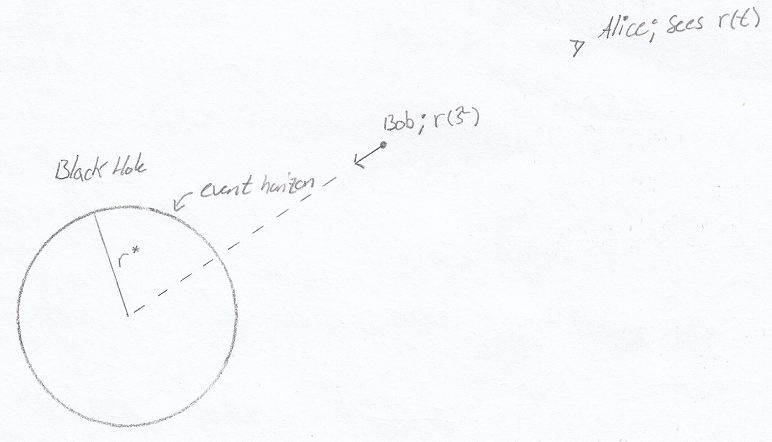
\includegraphics[width=0.8\textwidth]{figures//bh}
		\caption{The scenario with the black hole, Bob and Alice.}
		\label{fig:bh}
	\end{figure} 
	I can find $r(\tau)$ and $r(t)$ by using the variational principle. To this end I need the Lagrangian of the gravitational field. The Lagrangian is found from the metric, cf. equation \eqref{L1}, which is the Schwarzschild metric. The Schwarzschild metric describes the gravitational field from a spherically symmetric source, eg. a planet, star, black holes,.... It is given by
	\begin{equation}
		ds^2=-f(r)dt^2+f(r)^{-1}dr^2+r^2d\Omega^2,
	\end{equation} 
	where
	\begin{equation}
		f(r)=1-\frac{2MG}{r}.
	\end{equation}  
	Hereby the Lagrangian can be determined
	\begin{equation}
		L=-f(r)\dot{t}^2+f(r)^{-1}\dot{r}^2+r^2\dot{\theta}^2+r^2sin(\theta)^2\dot{\varphi}^2=-1.
	\end{equation} 
	Since I take Bob to fall in radially; $\dot{\varphi}=\dot{\theta}=0$. Hereby
	\begin{equation}
		L=-f(r)\dot{t}^2+f(r)^{-1}\dot{r}^2=-1.
	\end{equation} 
	From the Lagrangian I can determine the EOM of $t,r$ via the Euler-Lagrange equation. However, in this any most other cases, it is easier to combine the use of EOM's from the Euler-Lagrange equation and $L=-1$ - this last property is unique to GR. In this case it is (seen in hindsight) wise to begin with the EOM for the time-component
	\begin{equation}
		\frac{\partial L}{\partial t}-\frac{d}{d\tau}\bigg(\frac{\partial L}{\partial \dot{t}}\bigg)=0\Rightarrow \frac{d}{d\tau}\bigg(\underbrace{f(r)\dot{t}}_{\equiv \tilde{L}}\bigg)=0.
	\end{equation} 
	From the above I can determine $\dot{t}^2$ and insert it in $L$. Hereby
	\begin{equation}
		\tilde{L}^2-\dot{r}^2=f(r).
	\end{equation} 
	To solve this equation, I use that $L=const$ and that it can be evaluated in the limit of $r\Rightarrow\infty$. In this limit $f(r)\Rightarrow 1$ and $\dot{t}\Rightarrow1$, and so $\tilde{L}=1$. Hereby
	\begin{equation}
		\tilde{L}^2-\dot{r}^2=f(r)\Rightarrow \frac{dr}{d\tau}=-\sqrt{\frac{2MG}{r}},
	\end{equation} 
	where the minus sign comes from the fact that Bob is falling into the black hole - so it is directional. From the above I find via separation of variables
	\begin{equation}
		\sqrt{r}dr=-\sqrt{2MG}d\tau\Rightarrow r(\tau)\propto \tau^{\frac{2}{3}}.
	\end{equation} 
	The prefactor of $r(\tau)$ is not important in this case. What is important is the fact that there is no singularity at the event horizon. Bob experience himself falling through the event horizon without any changes. The question is now whether Alice will agree with Bob! To find $r(t)$ I use that
	\begin{equation}
		\frac{dr}{dt}=\frac{\dot{r}}{\dot{t}}=-\sqrt{\frac{2MG}{r}}\bigg(1-\frac{2MG}{r}\bigg).
	\end{equation} 
	In the limit of $r\Rightarrow 2MG$ the above differential equation has a solution on the form\footnote{Found by Taylor-expanding around $r=2MG$.}
	\begin{equation}
		r\approx 2MG+const\cdot e^{-\frac{t}{2MG}}.
	\end{equation} 
	What is noteworthy here is that as $t\Rightarrow \infty$ Alice will see Bob approach $r=2MG$, but never cross it! Hence, Bob and Alice will disagree on what transpires. This disagreement is due to time-dilation. 
\end{example}

\section{The Einstein equation}
The Einstein equation\index{Einstein equation} is the equation of motion for the metric, i.e. the gravitational field. The derivation of the Einstein equation revolves around the generalization of the classical equation that relates the gravitational field to the mass distribution; i.e. the Poisson equation
\begin{equation}
	\nabla^2\phi=4\pi G_N\rho.
\end{equation} 
In the relativistic limit the gravitational field and mass-energy is represented by the metric and energy-momentum tensor, respectively. Therefore, the starting point is an equation on the form
\begin{equation}
	f(g_{\mu\nu})=g(T_{\mu\nu}),
\end{equation} 
where $f$ and $g$ are \emph{some} functions of the metric and the (symmetric) energy-momentum tensor, respectively. Because $T^{00}=\rho$; $g\propto T_{\mu\nu}$. As for $f$; because of the classical limit it is expected that $f\supset \partial^2g^{\mu\nu}$. Further more, since the gravitational field can store energy, it is expected that field strength terms are included in $f$, i.e. $f\supset (\partial g_{\mu\nu})^2$. To be even more specific use that the mass-energy distribution curves space-time, so it is expected that $f$ is related to curvature. The curvature is measured by the Riemann curvature tensor that is defined in terms of the commutator of the covariant derivatives
\begin{equation}
	[D_\mu,D_\nu]V_\alpha\equiv R^\sigma_{\,\,\,\mu\beta\alpha}V_\sigma,
\end{equation} 
where
\begin{equation}
	R^{\sigma}_{\,\,\,\, \alpha \mu\beta}=\frac{\partial \Gamma^{\sigma}_{\alpha\mu}}{\partial x^{\beta}}-\frac{\partial \Gamma^{\sigma}_{\alpha\beta}}{\partial x^{\mu}}+\Gamma^{\eta}_{\alpha\mu}\Gamma^{\sigma}_{\beta\eta}-\Gamma^{\eta}_{\alpha\beta}\Gamma^{\sigma}_{\mu\eta}.
\end{equation} 
Because of Lorentz covariance $f$ cannot be directly proportional to $R^{\sigma}_{\,\,\,\, \alpha \mu\beta}$. Instead $f\sim g_{\sigma\mu}R^{\sigma}_{\,\,\,\, \alpha \mu\beta}=R^{\mu}_{\,\,\,\, \alpha \mu\beta}$ - where $R^{\mu}_{\,\,\,\, \alpha \mu\beta}=R_{\alpha\beta}$ is called the Ricci tensor. Therefore, a first guess about the form of the Einstein equation is
\begin{equation}
	R^{\mu}_{\,\,\,\, \alpha \mu\beta}\sim T_{\alpha\beta}.
\end{equation} 
However, as will be shown later on, the energy momentum tensor is the conserved Noether current associated with space-time translations in SR. This means\footnote{$,\mu$ denotes a partial derivative w.r.t. $\mu$. $;\mu$ denotes a covariant derivative w.r.t. $\mu$.}
\begin{equation}
	\text{SR:   }T^{\mu\nu}_{\,\,\,\,\,\,\, ,\mu}=0\Rightarrow \text{GR:   }T^{\mu\nu}_{\,\,\,\,\,\,\, ;\mu}=0.
\end{equation} 
This means that the covariant derivative of the Einstein equation should vanish. However, $R^{\mu\nu}_{\,\,\,\,\,\,\, ;\mu}\neq 0$, so $R^{\mu\nu}\propto T^{\mu\nu}$ is not the form of the Einstein equation. However, $f$ should still be related to the curvature in the form of the Ricci tensor. This conundrum is fixed by evaluating the covariant derivative of the Ricci tensor and subtracting the result - hence, a quantity related to the curvature will with a vanishing covariant derivative is obtained. The covariant derivative of the Ricci tensor can be evaluated by brute force, however this approach is a bit tedious since the Ricci tensor has four terms and the covariant derivative has three terms (an extra term since the covariant derivative is of a tensor with two indices). Instead use the Bianchi identity
\begin{equation}
	R_{\alpha\mu\nu\beta;\eta}+R_{\alpha\mu\eta\nu;\beta}+R_{\alpha\mu\beta\eta;\nu}=0.
\end{equation}  
Multiply this with $g^{\alpha\nu}$ and use that the covariant derivative of the metric vanishes. Hereby the metric can be pulled inside the covariant derivative to act on the Riemann curvature tensor. The result is given by
\begin{equation}
	R_{\mu\beta;\eta}-R_{\mu\eta;\beta}+R^\nu_{\,\,\,\mu\beta\eta;\nu}=0.
\end{equation}  
where the minus sign comes from permuting the outer indices of the Riemann curvature tensor. Multiplying once more with $g^{\mu\beta}$
\begin{equation}
	R_{;\eta}-R^ \beta_{\,\,\,\eta;\beta}-R^\nu_{\,\,\,\eta;\nu}=0.
\end{equation}  
Factorizing the covariant derivative and rewriting a bit
\begin{equation}
	\bigg(\frac{1}{2}\delta^\beta_{\,\,\,\eta}R-R^{\beta}_{\,\,\,\eta}\bigg)_;=0 \leftrightarrow \bigg(R^{\mu\nu}-\frac{1}{2}g^{\mu\nu}R\bigg)_;=0,
\end{equation}  
where $R$ is the Ricci scalar - the contracted version of the Ricci tensor. The last equality is what is needed for the Einstein equation! Therefore
\begin{equation}
	R^{\mu\nu}-\frac{1}{2}g^{\mu\nu}R\propto T^{\mu\nu},
\end{equation}  
where the LHS is defined as the Einstein tensor
\begin{equation}
	G^{\mu\nu}\equiv R^{\mu\nu}-\frac{1}{2}g^{\mu\nu}R.
	\label{ein1}
\end{equation} 
The proportionality constant can be found from the classical limit\footnote{Be careful here since there is a little conversion from $\phi$ to $g^{00}$ - As it turns out to be. See \citet{Cheng}.}. Hereby the Einstein equation is written as
\begin{equation}
	G^{\mu\nu}=-8\pi G_NT^{\mu\nu},
	\label{Einstein}
\end{equation} 
where the minus sign comes from the definition of the Ricci tensor. The Einstein equation, as it stands in equation \eqref{Einstein}, is however not completely generic, since the constraint that the LHS only contain second derivatives is a bit too strong. Higher derivatives would be suppressed too much, but a term proportional to the metric would be allowed as long as it vanishes in the classical limit. So, in the most generic form, to second order in the derivatives, the Einstein equation is given by
\begin{equation}
	G^{\mu\nu}+g^{\mu\nu}\Lambda=-8\pi G_NT^{\mu\nu}.
	\label{Einstein1}
\end{equation} 
$\Lambda$ is called the cosmological constant and it can be interpreted as a vacuum energy if it is moved to the RHS and taken as a contribution to the energy-momentum tensor. 
Equation \eqref{Einstein1} is the end product; it is the Einstein equation in its final form. The Einstein equation can be used to obtain the gravitational field from a given mass-energy distribution. The gravitational field can then be used in the geodesic equation to obtain the trajectories of particles in free fall in the gravitational field.  

\section{Standard Cosmology}
\label{SC}
\index{Standard cosmology}
The standard model of cosmology is built upon the FRW metric and the Friedmann equations derives therefrom. The FRW metric describes the gravitational field on cosmological scales, that is it describes the evolution of the universe as a whole. It is built from what is called the cosmological principle which approximates the universe as a perfect, spatially homogeneous, isotropic, fluid, as seen from the reference frame of a comoving observer\footnote{A comoving observer is one which is in free-fall in space-time, and for which the proper time is equal to the coordinate time, ie $g_{00}=-1$.}, on very large scales. The particles in the perfect fluid are taken to be the gravitationally bound objects in the universe. From these assumptions the metric is developed by writing down the most generic metric and then applying the physics of the cosmological principle to simplify the metric. \newline 
In general the metric depends on the choice of reference system. Taking the reference frame of the comoving observer the universe is approximated as isotropic. Since an isotropic universe has spherical symmetry the metric will be diagonal in these coordinates. Lastly, the homogeneous condition can be enforced in order to find~\citep{Weinberg1972}
\begin{equation}
	ds^2=-dt^2+R(t)^2\bigg[\frac{dr^2}{1-kr^2}+r^2d\Omega^2\bigg],
	\label{FRW}
\end{equation}  
where $d\Omega\equiv r^2d\theta^2+r^2sin(\theta)^2d\phi^2$, $r,\theta,\phi, t$ denotes radial coordinate, polar angle, azimuthal angle and time coordinate, respectively, $R(t)$ is a time-varying function called the scale factor and $k$ is a constant which sign is related to the curvature of the universe. To see how, consider different characteristics for $k, R(t)$:
\begin{enumerate}
	\item $k=0, R(t)=const\Rightarrow ds^2=-dt^2+R^2(dr^2+r^2d\Omega^2)$. Since $R=const$ it can be transformed away by a suitable coordinate transformation and the metric will thereby reduce to the Minkowski metric. The Minkowski metric results in a vanishing Riemann curvature tensor so, cf. Einsteins equation, the energy-momentum tensor will likewise vanish and there will be no matter in the universe. Hence, this is the case of an empty universe.
	
	\item $k=0, R(t)\neq const\Rightarrow ds^2=-dt^2+R^2(t)(dr^2+r^2d\Omega^2)$. Here $R(t)$ cannot be transformed away by a coordinate transformation, and even though the spatial part of the metric is flat, space-time is curved. Hence, the curvature tensor does not vanish, and the universe is not empty in this case. From observations $k\simeq 0$ and so this is a good approximation of the universe.
	
	\item $k>0, R(t)\neq const\Rightarrow ds^2=-dt^2+R(t)^2(\frac{dr^2}{1-|k|r^2}+r^2d\Omega^2)$. Once more $R(t)$ cannot be transformed away and space has a positive curvature. The spatial part of the metric resembles that of a 3D hypersphere. Since the hypersphere has a finite surface area, this universe is classified as a closed universe - referring to the finite size of the universe.
	
	\item $k<0, R(t)\neq const\Rightarrow ds^2=-dt^2+R(t)^2(\frac{dr^2}{1+|k|r^2}+r^2d\Omega^2)$. Here the spatial part of the metric resembles that of a 3D pseudo hypersphere. Since the pseudo hypersphere has infinite volume, the universe is classified as open - referring to the infinite size of the universe.
	
\end{enumerate}
By using the metric in the Einstein equation the Friedmann equations can be found. Neglecting the vacuum energy, equation \eqref{ein1} and \eqref{Einstein} can be combined to write the Einstein equation as follows
\begin{equation}
	R^{\mu\nu}-\frac{1}{2}g^{\mu\nu}R=-8\pi G_NT^{\mu\nu}.
	\label{E1}
\end{equation} 
Because the Ricci tensor includes a lot of terms the Einstein equation is often rewritten by eliminating Ricci scalar and instead introducing the trace of the energy-momentum tensor. This is done by taking the trace on both sides of equation \eqref{E1}. Hereby
\begin{equation}
	R^{\mu\nu}=-8\pi G_N(T^{\mu\nu}-\frac{1}{2}g^{\mu\nu}T^{\alpha}_{\,\,\,\alpha}).
	\label{E2}
\end{equation}  
To obtain the equations for $R(t)$ use equation \eqref{FRW} in equation \eqref{E2} to determine the Ricci tensor and use that the energy-momentum tensor for a perfect fluid is given by
\begin{equation}
	T^{\mu\nu}=Pg^{\mu\nu}+(P+\rho)u^\mu u^\nu,
\end{equation} 
where $P$ is the pressure of the fluid, $\rho$ is the energy density of the fluid and $u$ is the four-velocity. The energy-momentum tensor is the conserved Noether current associated with space-time translations in Sr. Therefore the relativistic divergence of the energy-momentum tensor must vanish in SR. Generalizing from SR to GR the derivative is generalized to th covariant derivative. Therefore
\begin{equation}
	T^{\mu\nu}_{\,\,\,\,\,\, ; \nu}=0.
	\label{T1}
\end{equation} 
The $\mu=0$ component of equation \eqref{T1} reveals
\begin{equation}
	d(\rho R^3)=-Pd(R^3)\rightleftarrows \dot{\rho}+3H(\rho +P)=0,
	\label{T2}
\end{equation}  
where $H\equiv \frac{\dot{R}}{R}$. Equation \eqref{T2} implies that the expansion of the universe can leads to local changes in the energy density. Note that the space-time geometry can hold energy and so energy can flow between it and matter - hence the energy of the space-time geometry has to be counted if one is to consider energy conservation. Taking $E=\rho V$ and $R^3\sim V$ equation \eqref{T2} can be rewritten as follows
\begin{equation}
	dE+pdV=0.
	\label{E3}
\end{equation} 
Equation \eqref{E3} is the first law of thermodynamics with no heat exchange ($dQ=0$). Hence, cf. equation \eqref{E3}, the FRW metric implies that the universe expands adiabatically ($dQ=0$). Approximating the processes that occur to be reversible means the expansion is also isentropic, i.e.$dQ_{rev}=TdS=0\Rightarrow dS=0$. The approximation of reversible processes is equivalent to the approximation of local thermal equilibrium in the universe. It is important to emphasize this approximation since it is key in the established formalism that treats DM.\newline
Using $P=w\rho$ with $w=const$ in equation \eqref{T2} reveals $\rho\propto R^{-3(1+w)}$. $w$ depends on which component dominates the universe. The popular considerations are radiation ($w=\frac{1}{3}$), matter ($w=0$) and vacuum energy ($w=-1$)
\begin{equation}
	\begin{split}
		\text{Radiation:} \quad &\rho\propto R^{-4},\\
		\text{Matter:} \quad &\rho\propto R^{-3},\\
		\text{Vacuum energy:} \quad &\rho=const.\\
	\end{split}
\end{equation}  
In this thesis the early universe, which was radiation dominated, will primarily be considered and so $\rho\propto R^{-3}$ will often be assumed. By evaluating the different components of equation \eqref{E2}; One from the $00$-component and one from the $ij$-components
\begin{equation}
	\bigg(\frac{\dot{R}}{R}\bigg)^2\equiv H^2=\frac{8\pi G_N}{3}\rho-\frac{k}{R^2}, \qquad \frac{\ddot{R}}{R}=-\frac{4\pi G_N}{3}(\rho+3P).
	\label{fried}
\end{equation} 
Equation \eqref{fried} defines the Friedmann equations (the first to the left) which describe the relationship between curvature, matter density, pressure and the expansion of the universe. The first Friedmann equation is often rewritten by defining $\rho_c\equiv \frac{3H^2}{8\pi G_N}$. Hereby
\begin{equation}
	H^2=\frac{8\pi G_N}{3}\rho-\frac{k}{R^2}\Rightarrow \frac{k}{H^2R^2}=\Omega-1,
	\label{f1}
\end{equation} 
where $\Omega\equiv \frac{\rho}{\rho_c}$. Since $k\simeq 0$ is observed it is clear from equation \eqref{f1} that $\Omega\simeq 1$.